\chapter{Systematics uncertainties on angular observables and results}

In the following sections are explained the five main sources of systematic uncertainties that are considered for the $A_{FB}$ measurement.

\subsection{Non-flat angular efficiency}

The angular efficiency is non-flat as a function of $\cos\theta_\ell$ and $\cos \theta_\Lambda$.
Therefore, while integrating the full angular distribution, terms that cancel with perfect efficiency may
remain and generate a bias in the final result. In order to deal with this effect we generate events
in a 2D ($\cos\theta_\ell$,$\cos \theta_\Lambda$) space using the theoretical distribution described by
Eq.\ref{eq:2DcosThetaLandB} multiplied by the 2D efficiency histogram reported in Fig.~\ref{fig:2DcosThetaLandBeff}.
Then we take 1-dimensional projections and we fit them with the default 1D efficiency function.
In Fig.~\ref{fig:effBias} are shown the deviations from the true generated value $\Delta x = x_{true} - x_{measured}$.
Since the mean of these distributions is non zero by more then 3$\sigma$, we take it as a systematic error.

\begin{figure}
\centering
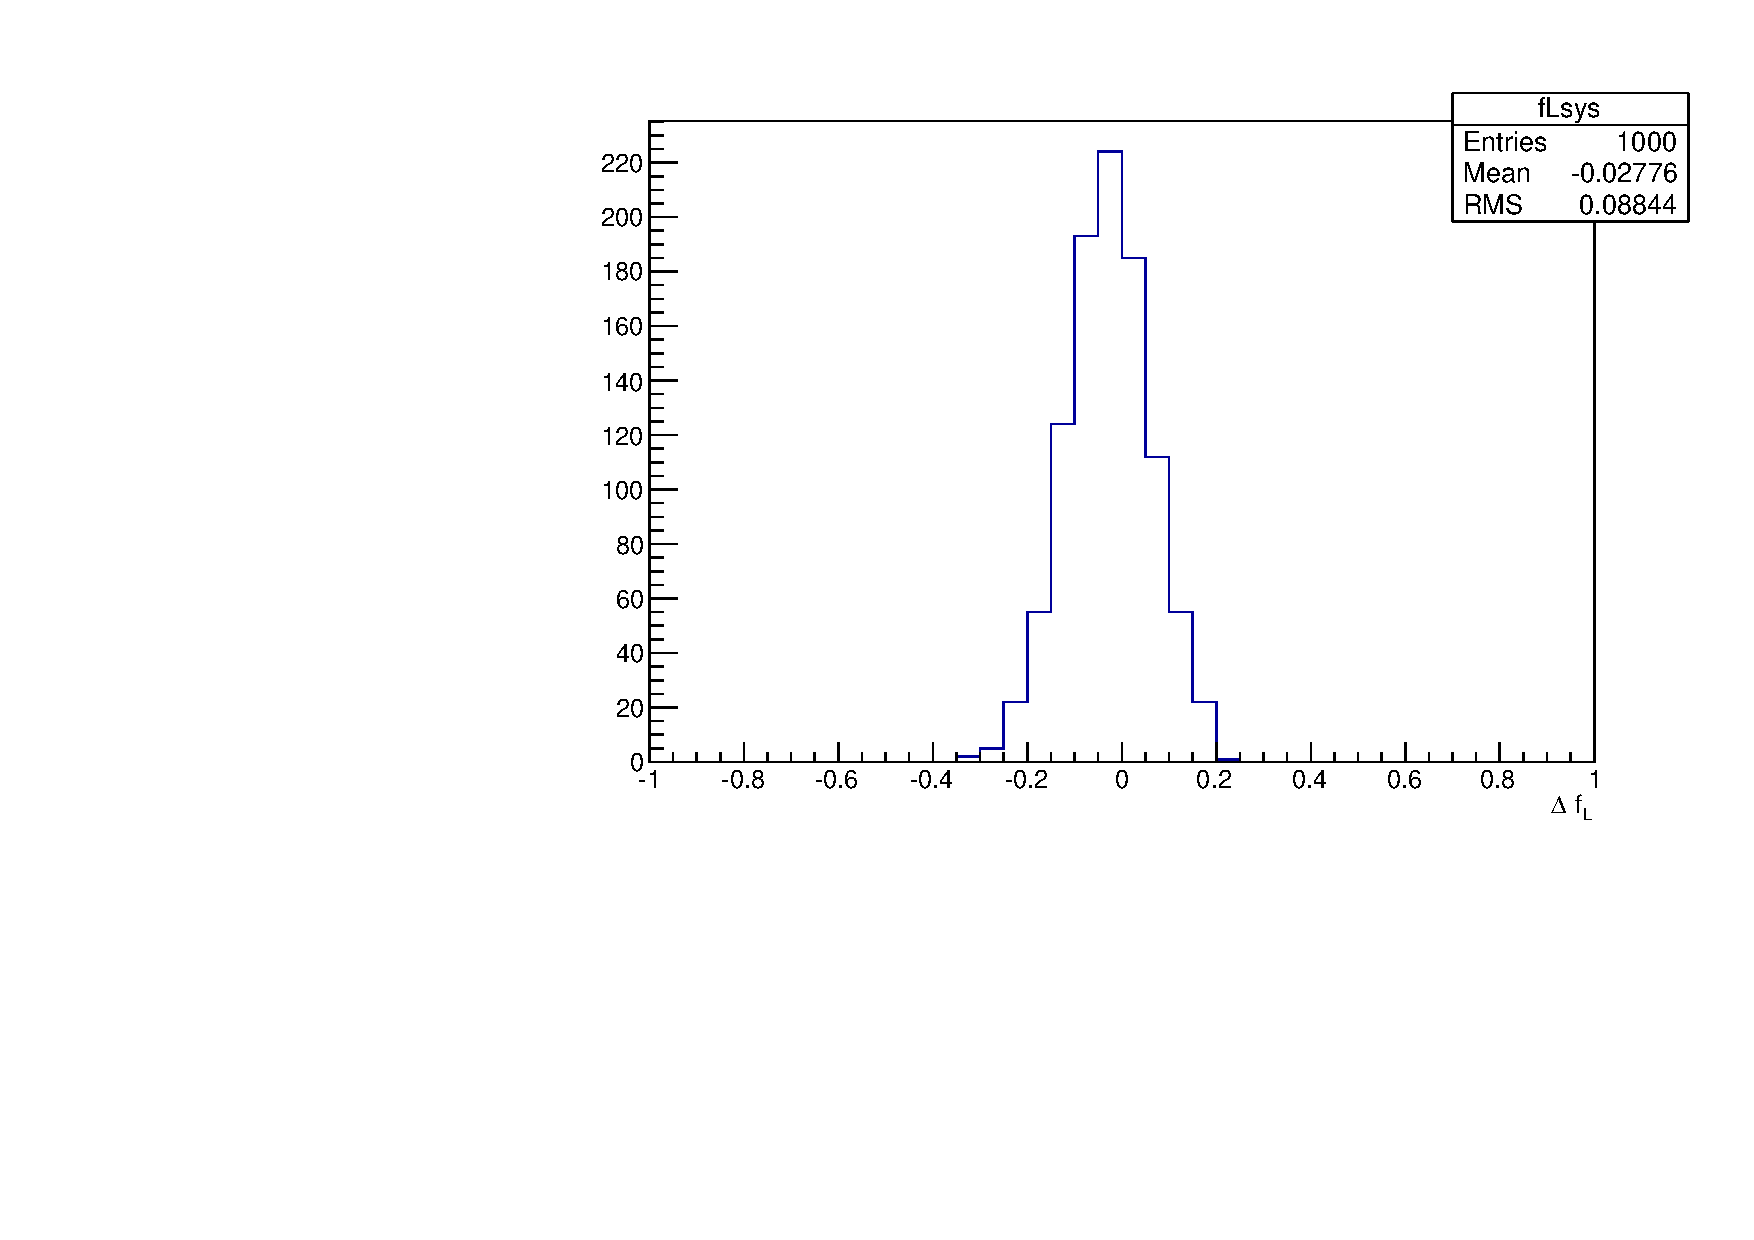
\includegraphics[width=0.45\textwidth]{Lmumu/figs/fLsys_efficiency.pdf}
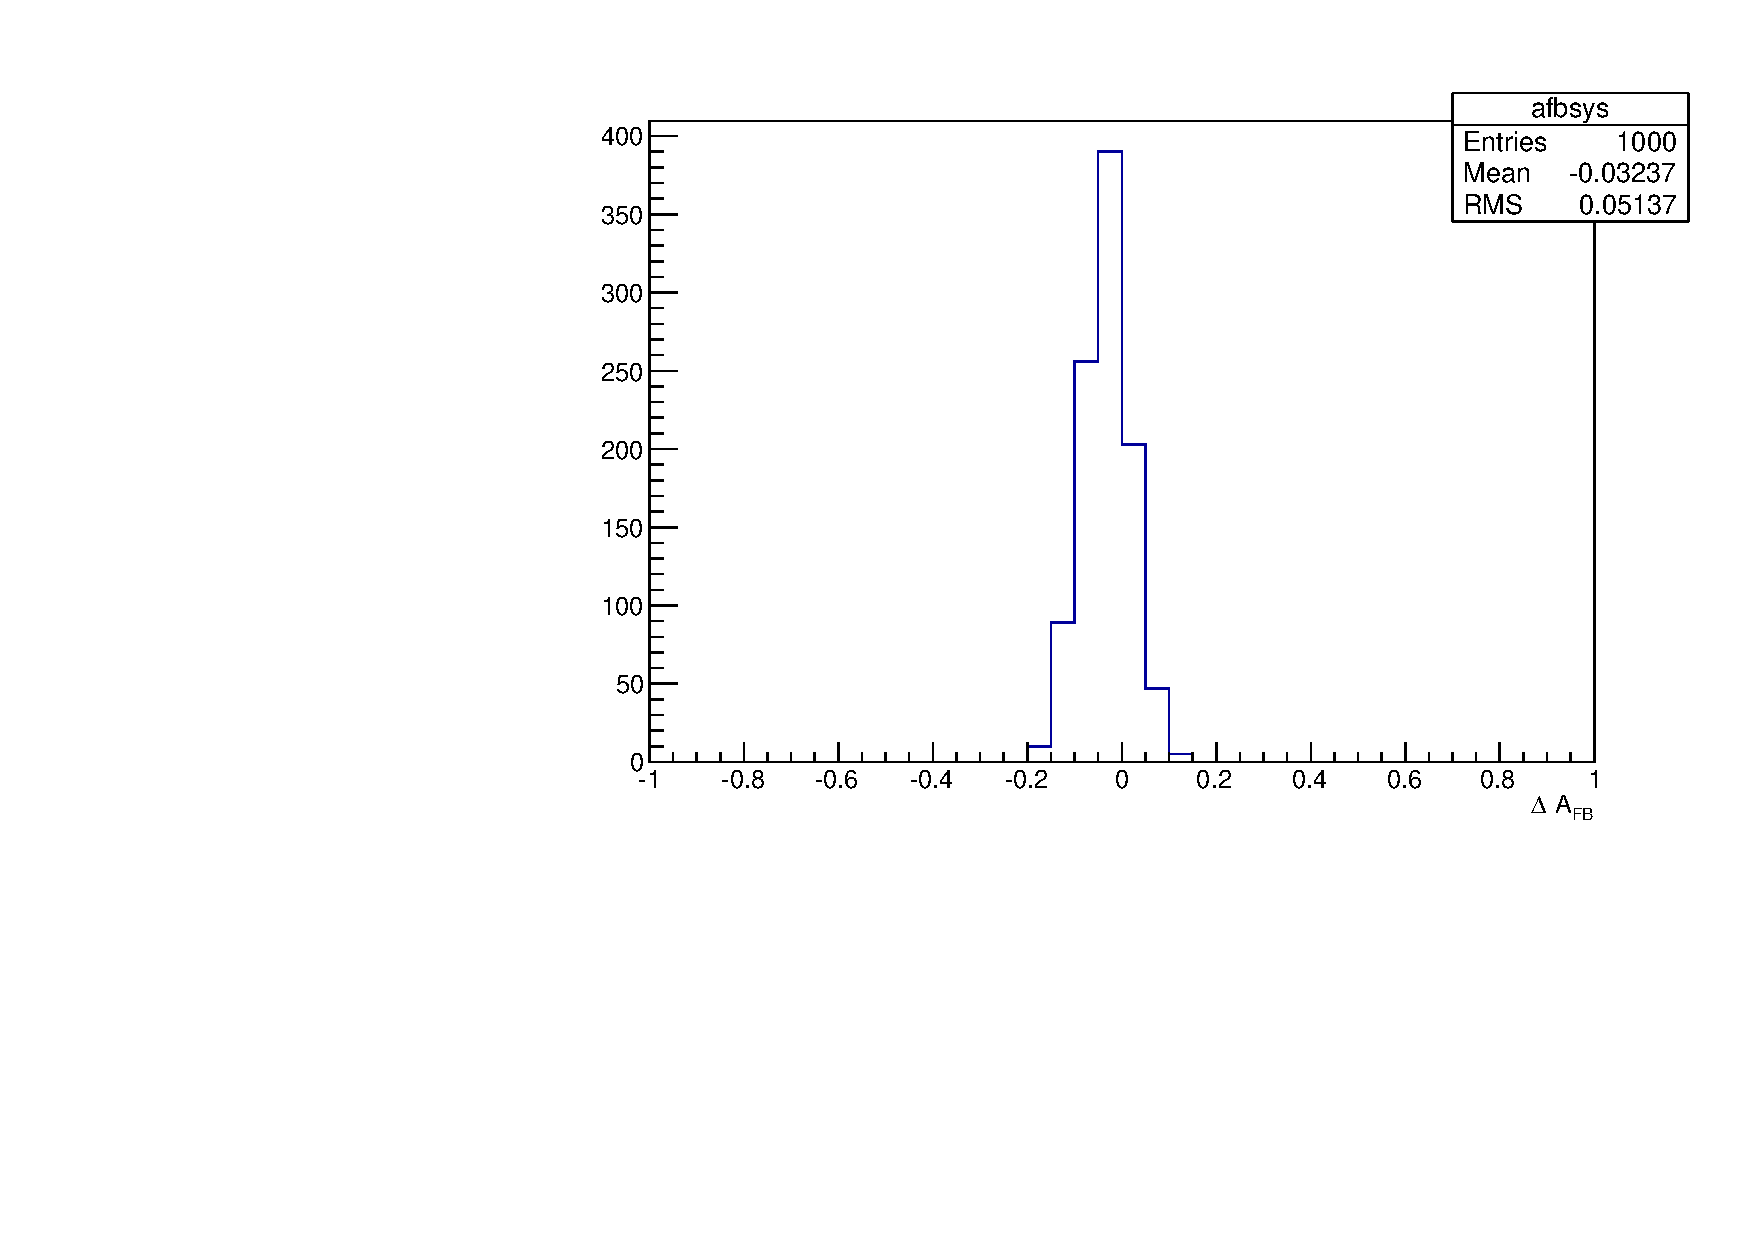
\includegraphics[width=0.45\textwidth]{Lmumu/figs/afbsys_efficiency.pdf}
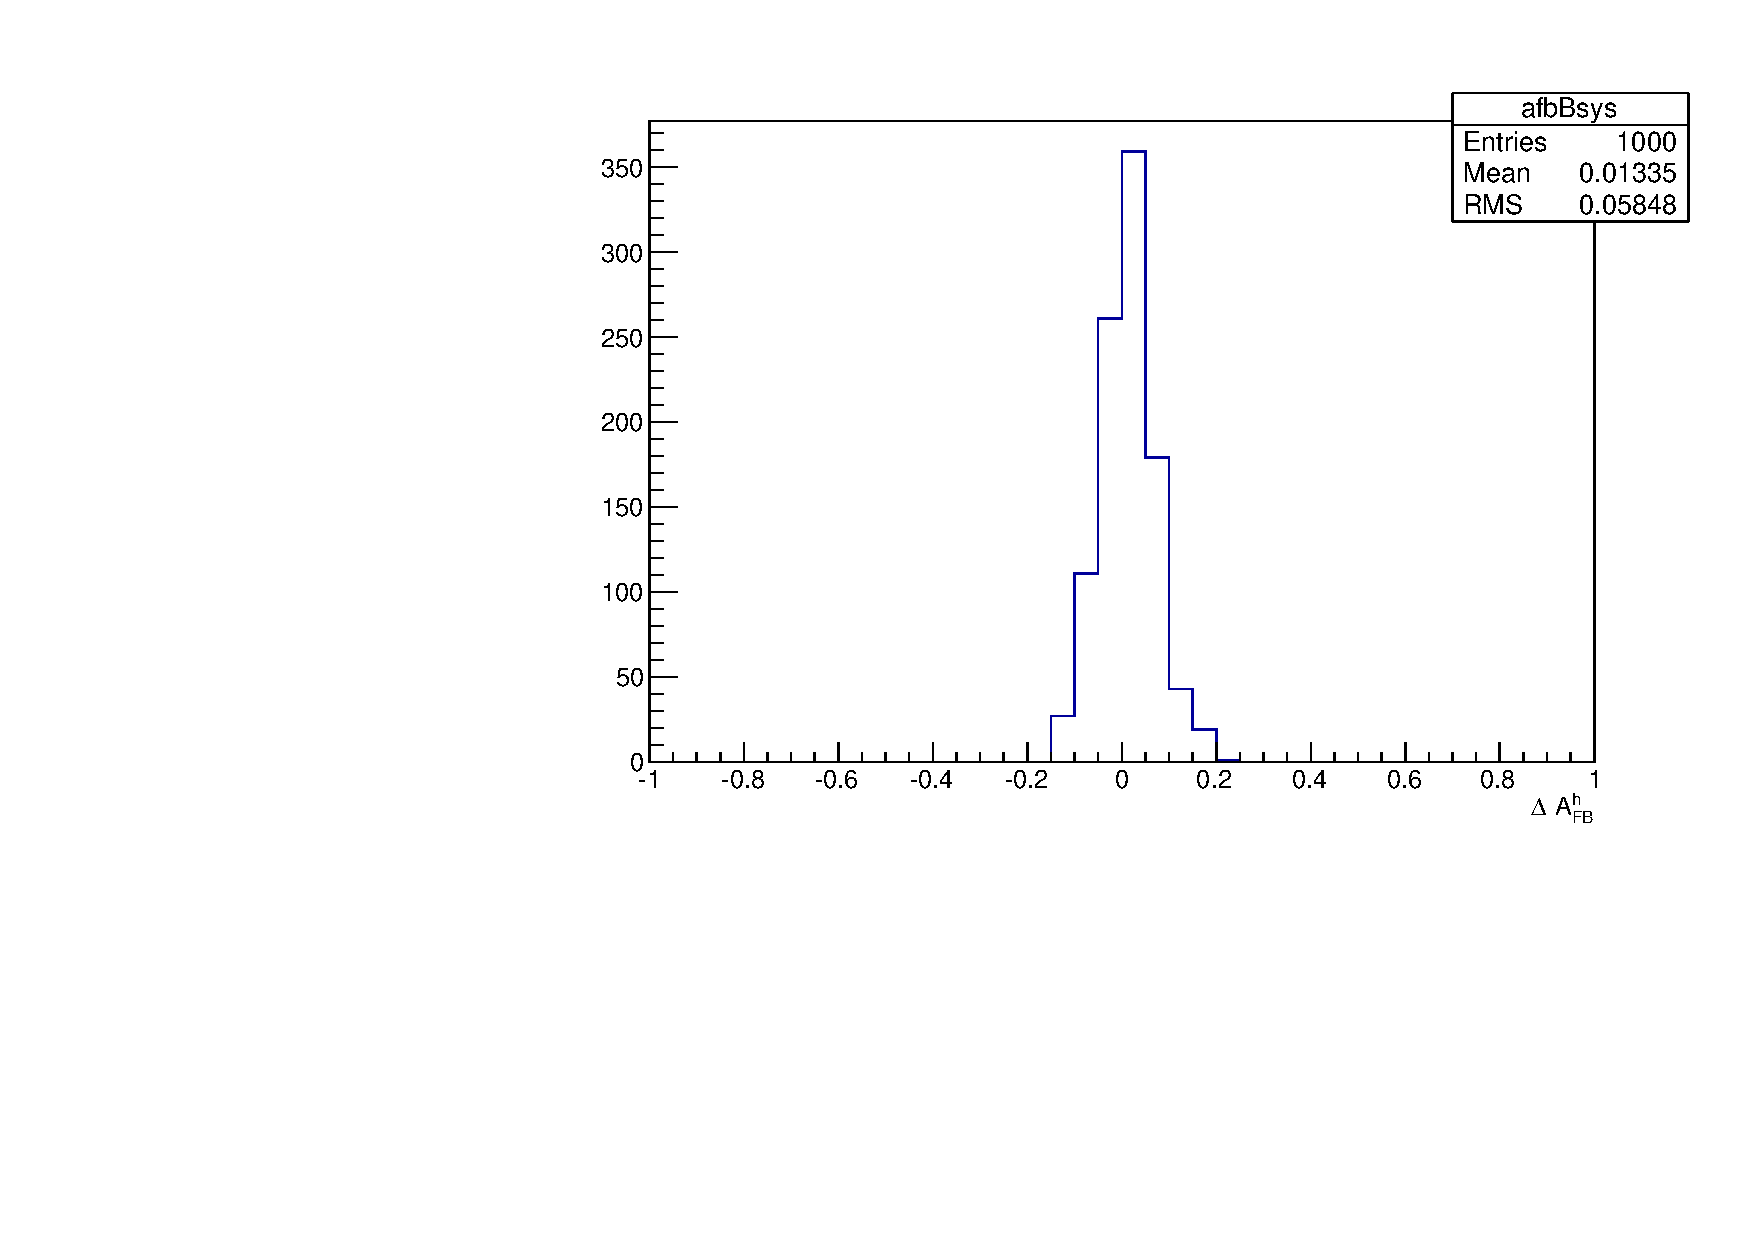
\includegraphics[width=0.45\textwidth]{Lmumu/figs/afbBsys_efficiency.pdf}
\caption{Plots show the absolute difference of the observables' values obtained fitting toy MC generated with a 2D distributions multiplied by a 2D efficiency and fitting 1D projections. From left to right for $f_L$, $A_{FB}^\ell$ and $A_{FB}^h$. }
\label{fig:effBias}
\end{figure}




\subsection{Resolution}

We investigated whether the angular resolution can bias the $A_{FB}$ measurement.
If the angular distribution is asymmetric, a non-zero resolution may yield to an asymmetric migration of events,
which can then generate a bias in the value of $A_{FB}$.
This is especially important for $\cos \theta_\Lambda$, which has worse resolution and a considerably asymmetric distribution.
In order to study this systematic we used toy experiments where events are generated following the measured distributions (including efficiencies).
Then these events are normally smeared by the angular resolution. To be conservative we always use the case with biggest angular resolution,
down-down events, as reported in table \ref{tab:resolutions}.
Finally, the smeared and not-smeared distributions are fitted with the same angular pdf.  
The average deviations from the default values are reported in table \ref{tab:resolSys} as a function of \qsq.
All are are several $\sigma$ away from 0, therefore we assign these average deviations as systematics.


\begin{table}[h]
\centering
\begin{tabular}{c|c|c|c|c|c}
 \qsq bin &  $\sigma_\ell$    &  $\sigma_\Lambda$   & $\Delta A_{FB}^\ell$ &  $\Delta f_{L}$ & $\Delta A_{FB}^h$ \\ \hline
0.1-2.0  & 0.0051 & 0.061 & 0.0011 & -0.0022 & -0.007 \\ 
11.0-12.5 & 0.0055 & 0.067 & 0.0016 & -0.0051 & -0.013 \\
15.0-16.0 & 0.0059 & 0.070 & 0.0006 & -0.0054 & -0.010 \\
16.0-18.0 & 0.0064 & 0.070 & 0.0014 & -0.0077 & -0.010 \\
18.0-20.0 & 0.0081 & 0.074 & 0.0014 & -0.0062 & -0.010 \\
\hline
15.0-20.0 & 0.0066 & 0.072 & 0.0013 & -0.0076 & -0.011 \\
\end{tabular}
\caption{Values of simulated $\cos\theta_\ell$ and $\cos\theta_\Lambda$ resolutions and systematics on angular observables in bins of \qsq.}
\label{tab:resolSys}
\end{table}


\subsection{Angular efficiency}

Selection requirements on the minimum momentum of the muons has the effect of warping the $\cos \theta_\ell$ distribution
removing candidates with extreme values of $\cos \theta_\ell$. And similarly the impact parameter requirements affect $\cos \theta_\Lambda$
as very forward hadrons tend to have lower IP.
An imprecise determination of the reconstruction and selection efficiency can introduce extra oddity and therefore bias the $A_{FB}$ measurement.
In particular the baryon side distribution is asymmetric and the correct evaluation of this asymmetry is important to avoid biases in $A_{FB}^h$.

In order to asses this systematic we remove the kinematic re-weighting of the MC described in sec.\ref{sec:kinWeight}
and we check what is the effect on the observables measurement.
We do this by fiting toy samples using the same theoretical pdf multiplied by the efficiency funcion obtained with and without kinematical reweight.
Finally, we take the average bias on the final results over 1000 toy experiments as a systematic. Results are shown in table \ref{tab:AfbeffSys}.

\begin{table}[h]
\centering
\begin{tabular}{c|c|c|c}
 \qsq bin  & $A_{FB}^h$   & $A_{FB}^\ell$ & $f_L$ \\ \hline
0.1-2.0    &  0.0093 & 0.0020  & 0.0440 \\ 
11.0-12.5  &  0.0069 & 0.0069  & 0.0027 \\
15.0-16.0  &  0.0109 & 0.0018  & 0.0046 \\
16.0-18.0  &  0.0159 & 0.0012  & 0.0043 \\
18.0-20.0  &  0.0148 & 0.0030  & 0.0017 \\
\hline
15.0-20.0  &  0.0138 & 0.0002  & 0.0046 \\
\end{tabular}
\caption{Values systematic erros due to limited knowledge of the efficiency function on the three angular observables in bins of \qsq}
\label{tab:AfbeffSys}
\end{table}

Furthermore, we take in account for the effect of the limited MC statistics. This is not already taken in account
by the Feldman-Cousins plug-in method ( see \ref{sec:FeldmanCousins}) since the efficiency parameters are always fixed
in the fit. We generate toy MC events using the measured values of angular observables and the default efficiency. 
Then we vary the efficiency with its errors and we refit with the new efficiency model. In each toy we generate a number
of events comparable to the one we have in data in bins of \qsq. The average deviation over 1000 toys is taken as systematic,
values are reported in table \ref{tab:stateffsys}. N.B.: Efficiency parameters are always fixed when fitting the angular distributions. 

Finally, we checked polarisation effects of the efficiency description by varying the polarisation parameter in the MC weighting
 from $- \sigma$ to $+ \sigma$ for the central measured value, as done for the branching ratio analysis \ref{sec:BRpolsys}. 
 Then again we generate toys and fit them using efficiency models obtained using with different values of polarisation. 
 No significant effect is found on the final results so we don't assign extra systematics. 

\begin{table}[h]
\centering
\begin{tabular}{c|c|c|c}
 \qsq bin  & $A_{FB}^\ell$   & $f_{L}$ & $A_{FB}^h$ \\ \hline
0.1-2.0    &  0.00151 & 0.00170  & 0.00213 \\
11.0-12.5  &  0.00121 & 0.00154  & 0.00196 \\
15.0-16.0  &  0.00004 & 0.00017  & 0.00103 \\
16.0-18.0  &  0.00065 & 0.00246  & 0.00417 \\
18.0-20.0  &  0.00023 & 0.00372  & 0.00162 \\
\hline
15.0-20.0  &  0.00039 & 0.00091  & 0.00137 \\
\end{tabular}
\caption{Values systematic erros due to MC statistics on the three angular observables in bins of \qsq}
\label{tab:stateffsys}
\end{table}


\subsection{Background parameterisation}
\label{sec:bkgShapeSys}

Since there is a certain degree of arbirariety in the choice of a parameterisation for the background, especially in bins with low statistics,
we study if this may be a source of systemaitcs. We generate toy MC experiments using the shapes from real data fits and same statistics as in each \qsq bin.
Then we fit each toy with 2 models: the default one, a "line times efficiency" function as descibed in \ref{sec:BkgParam}, and a "flat times efficiency" function. We take the average bias over 100 toys as systematic.
%This is currently our biggest systematic and it is on average at the level of 30\% of the statistical error or less.
%So this results uncertainty is still dominated by statistics.
Results are reported in table \ref{tab:bkgParamSys}. The most affected observable is $f_L$, while the least affected is $A_{FB}^\ell$. 

%Finally, we consider also the bias which may be cause by fixing the background fraction in the fit by fitting the same toys with
%a model where the background fraction is fixed to a random value normally distributed around the measured one. This systematic is negligible
%compared to the previous one but we add it anyway to the final systematic.
%The total result calculated as the square root sum of the 2 compoents is reported in table \ref{tab:bkgParamSys}.


\begin{center}
\begin{table}[h]
\centering
\begin{tabular}{l|c|c|c}
\hline
\qsq bin & $A_{FB}^\ell$     & $f_L$      & $A_{FB}^h$   \\ \hline
0.1-2.0         &  0.003	 &   0.049	  &  0.053		\\
11.0 - 12.5		&  0.045     &   0.034	  &  0.035     \\
15.0 - 16.0 	&  0.010     &   0.038    &  0.026     \\
16.0 - 18.0 	&  0.026     &   0.036    &  0.022     \\
18.0 - 20.0 	&  0.011     &   0.031    &  0.025     \\
\hline
15.0 - 20.0		&  0.007     &   0.014    &  0.017     \\
\hline
\end{tabular}
\caption{ Values of systematics due to the choice of background parameterisation in bins of \qsq. }
\label{tab:bkgParamSys}
\end{table}
\end{center}




\subsection{Polarisation}

To study the effect of a non-zero $\Lambda_b$ production polarisation we generate events using the distributions \ref{eq:lepton2D} and \ref{eq:hadron2D} as a function of our angular observable and $\cos\theta$, which is sensitive to polarisation.
Similarly to the procedure we used for the branching ratio measurement, we generate events for three values of the polarisation corresponding to $\pm \sigma$ from the recent LHCb measurement and its central value ($Pb = 0.06 \pm 009$ \cite{Aaij:2013oxa}).
In the theoretical distributions $\cos \theta$ is always odd therefore with perfect efficiency it always drops out by integrating over $\cos\theta$.
Therefore the generated distributions contain also the information of the 2-dimensional efficiency. In fig \ref{fig:2Deffs} are reported 2D efficiencies as a function of $\cos \theta_\ell$ and $\cos \theta_\Lambda$ versus $\cos \theta$. And in fig \ref{fig:Afbpolsys} are reported distributions of the absolute difference between the observable value obtained fitting generated events with the two polarisation values. 
%We then plot the the biggest difference between the plus or minus $\sigma$ case and the central value.
For the integrated high \qsq region we obtain the following average deviations: $\Delta f_L = 0.0016 \pm 0.0012$, $\Delta A_{FB}^\ell = 0.00048 \pm 0.00074$ and $\Delta A_{FB}^h = 0.00014 \pm 0.00075$.
Since all average differences are consistent with zero within less than 1.5$\sigma$ we do not assign extra systematics for polarisation.

\begin{figure}
\centering
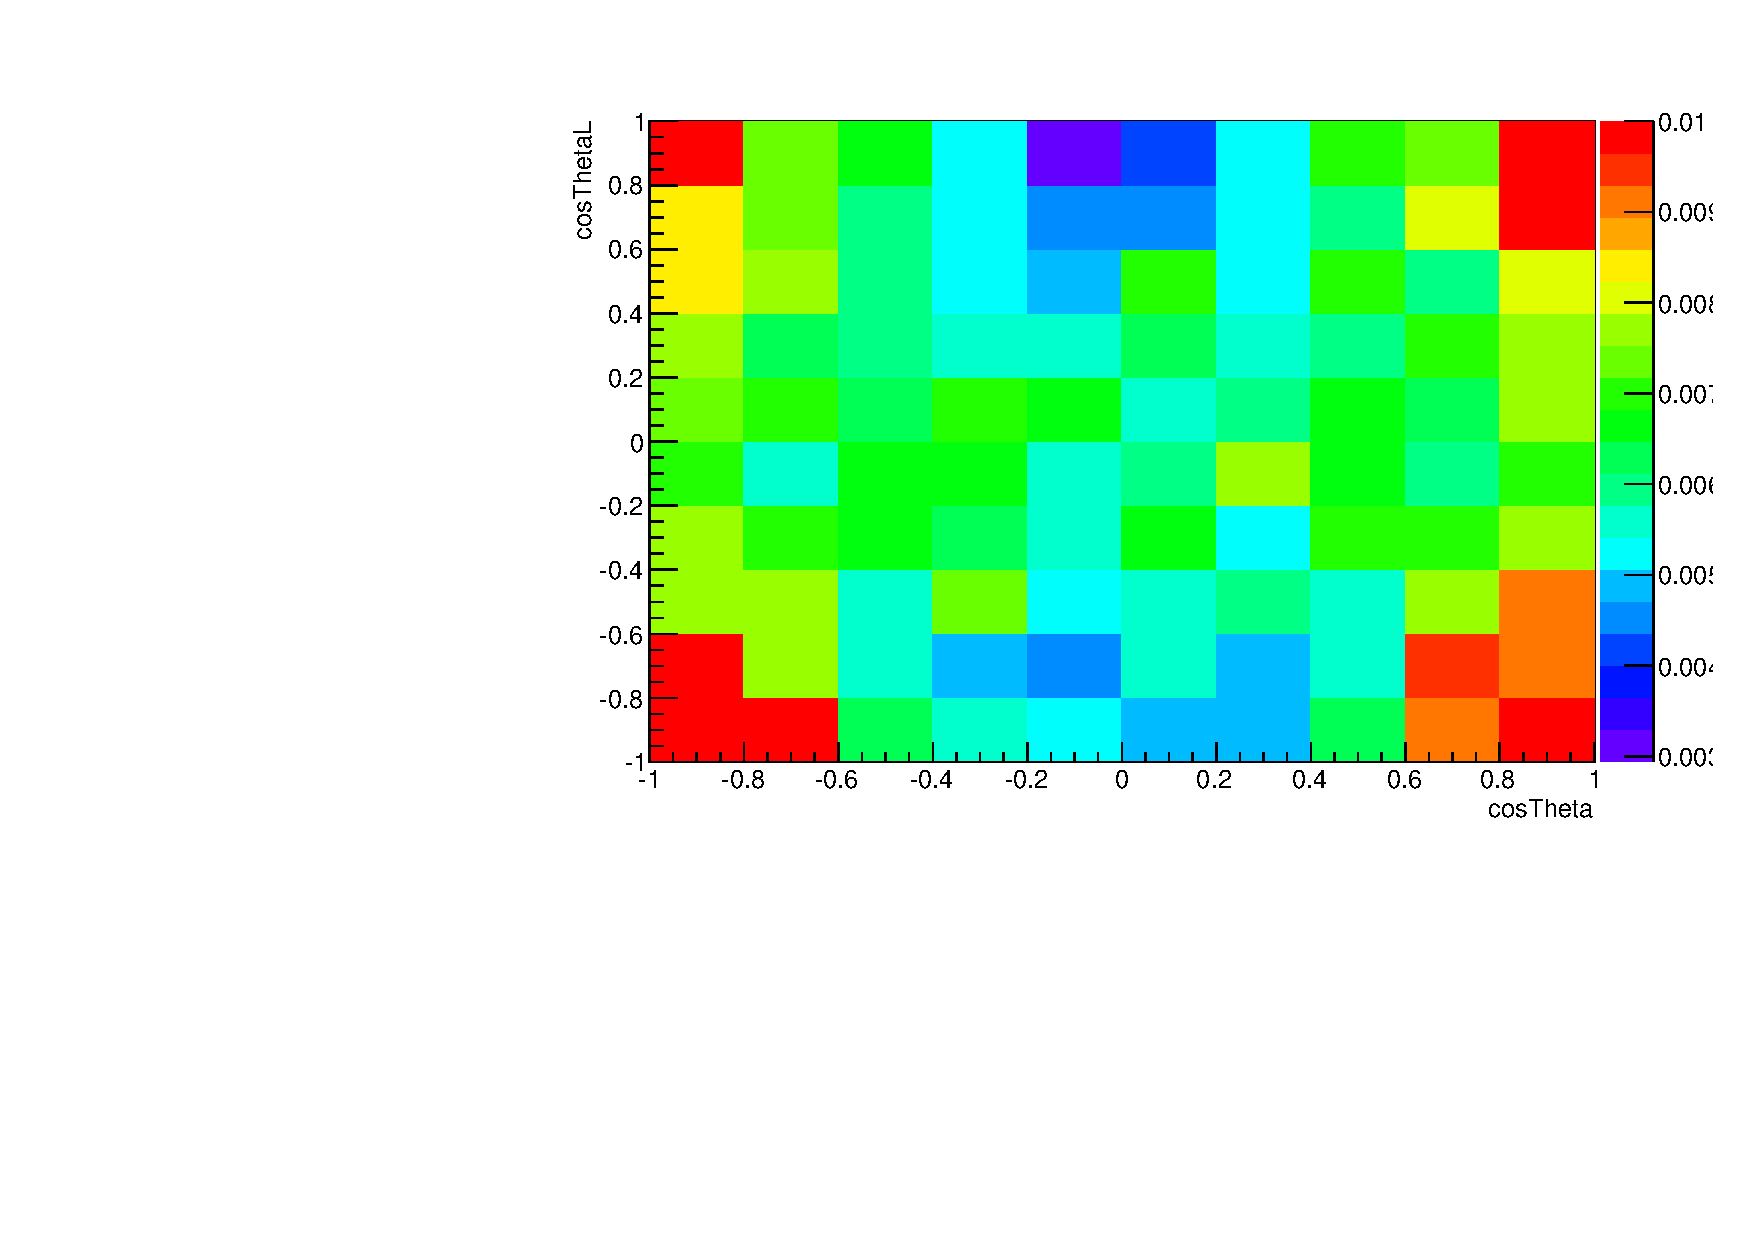
\includegraphics[width=0.45\textwidth]{Lmumu/figs/2Deff_tot_cosThetaL_vs_cosTheta_All.pdf}
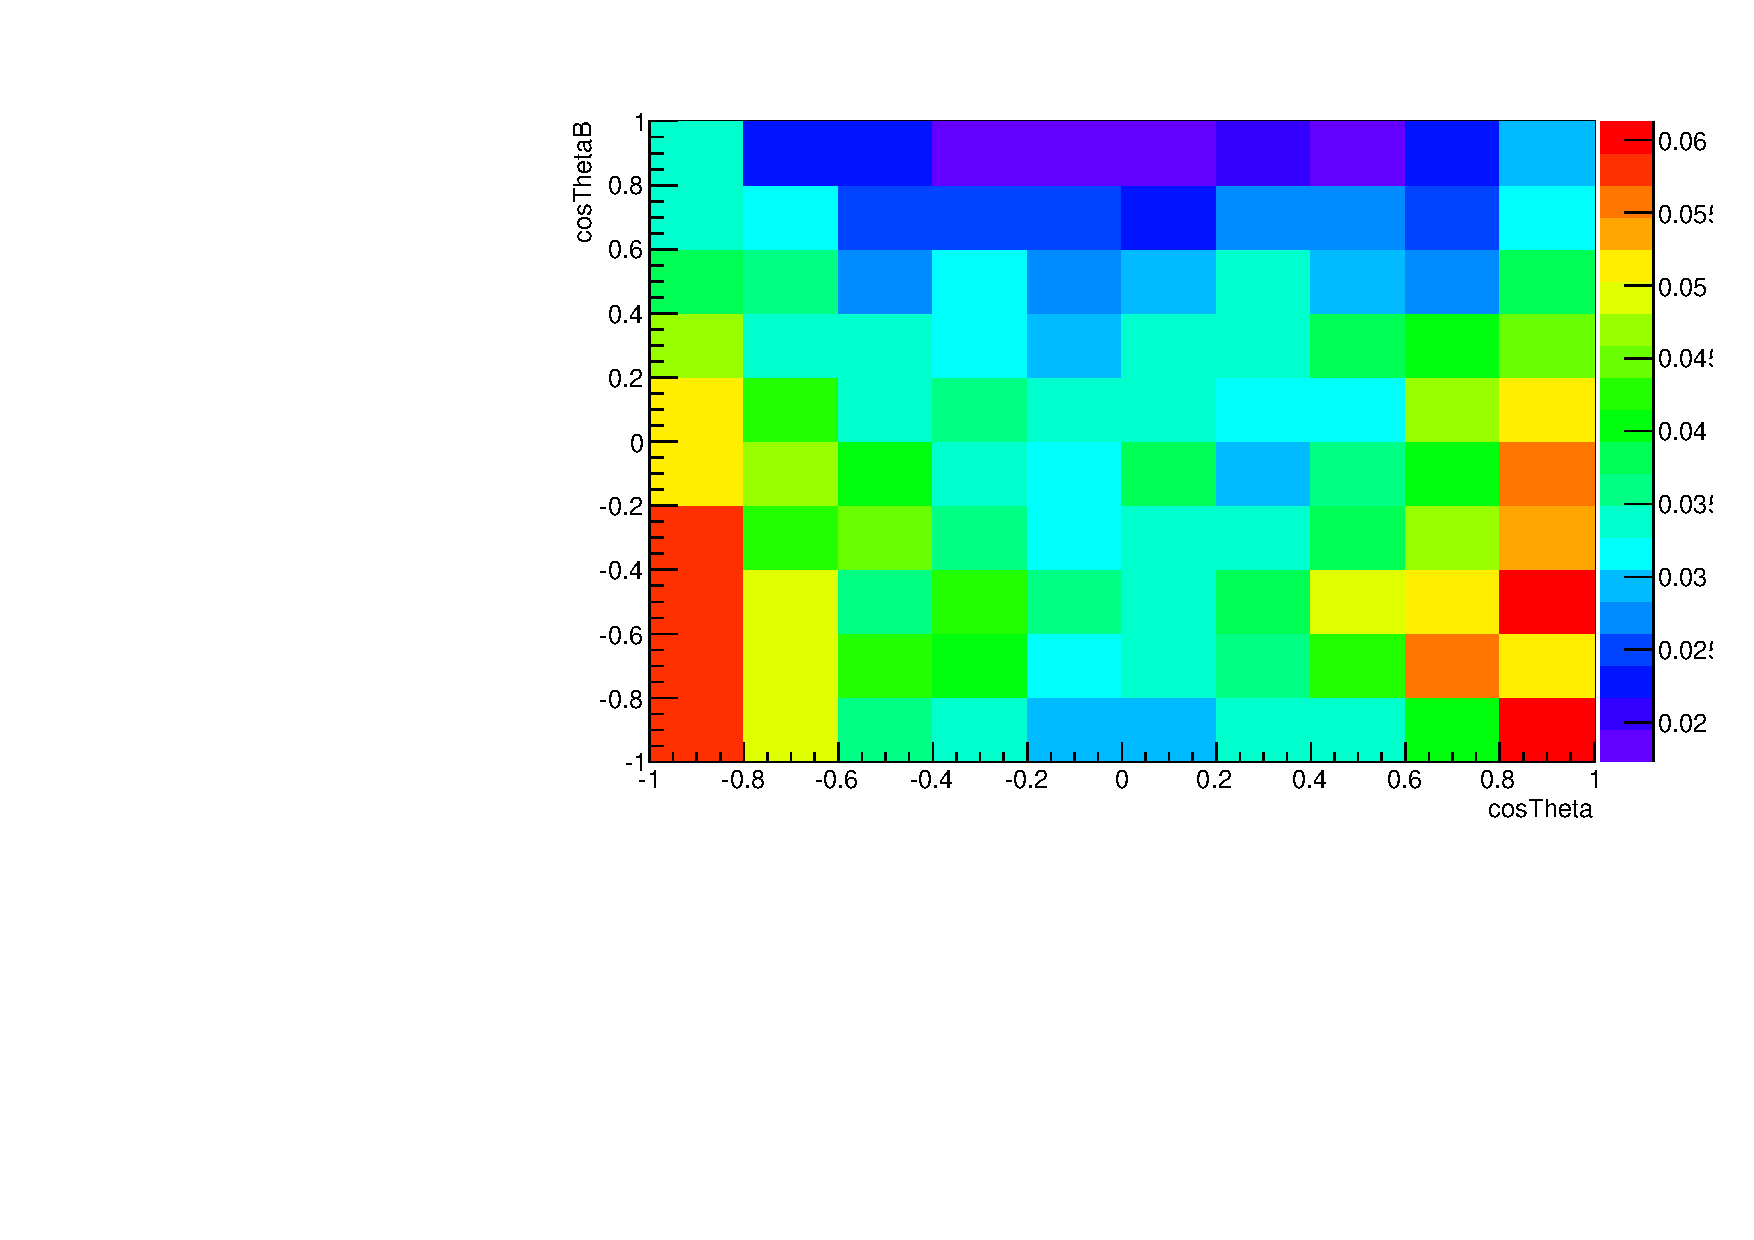
\includegraphics[width=0.45\textwidth]{Lmumu/figs/2Deff_upper_cosThetaB_vs_cosTheta_All.pdf}
\caption{2-dimensional efficiencies obtained from weighted MC for $\cos \theta_\ell$ and $\cos\theta_\Lambda$ versus $\cos\theta$.}
\label{fig:2Deffs}
\end{figure}
\begin{figure}
\centering
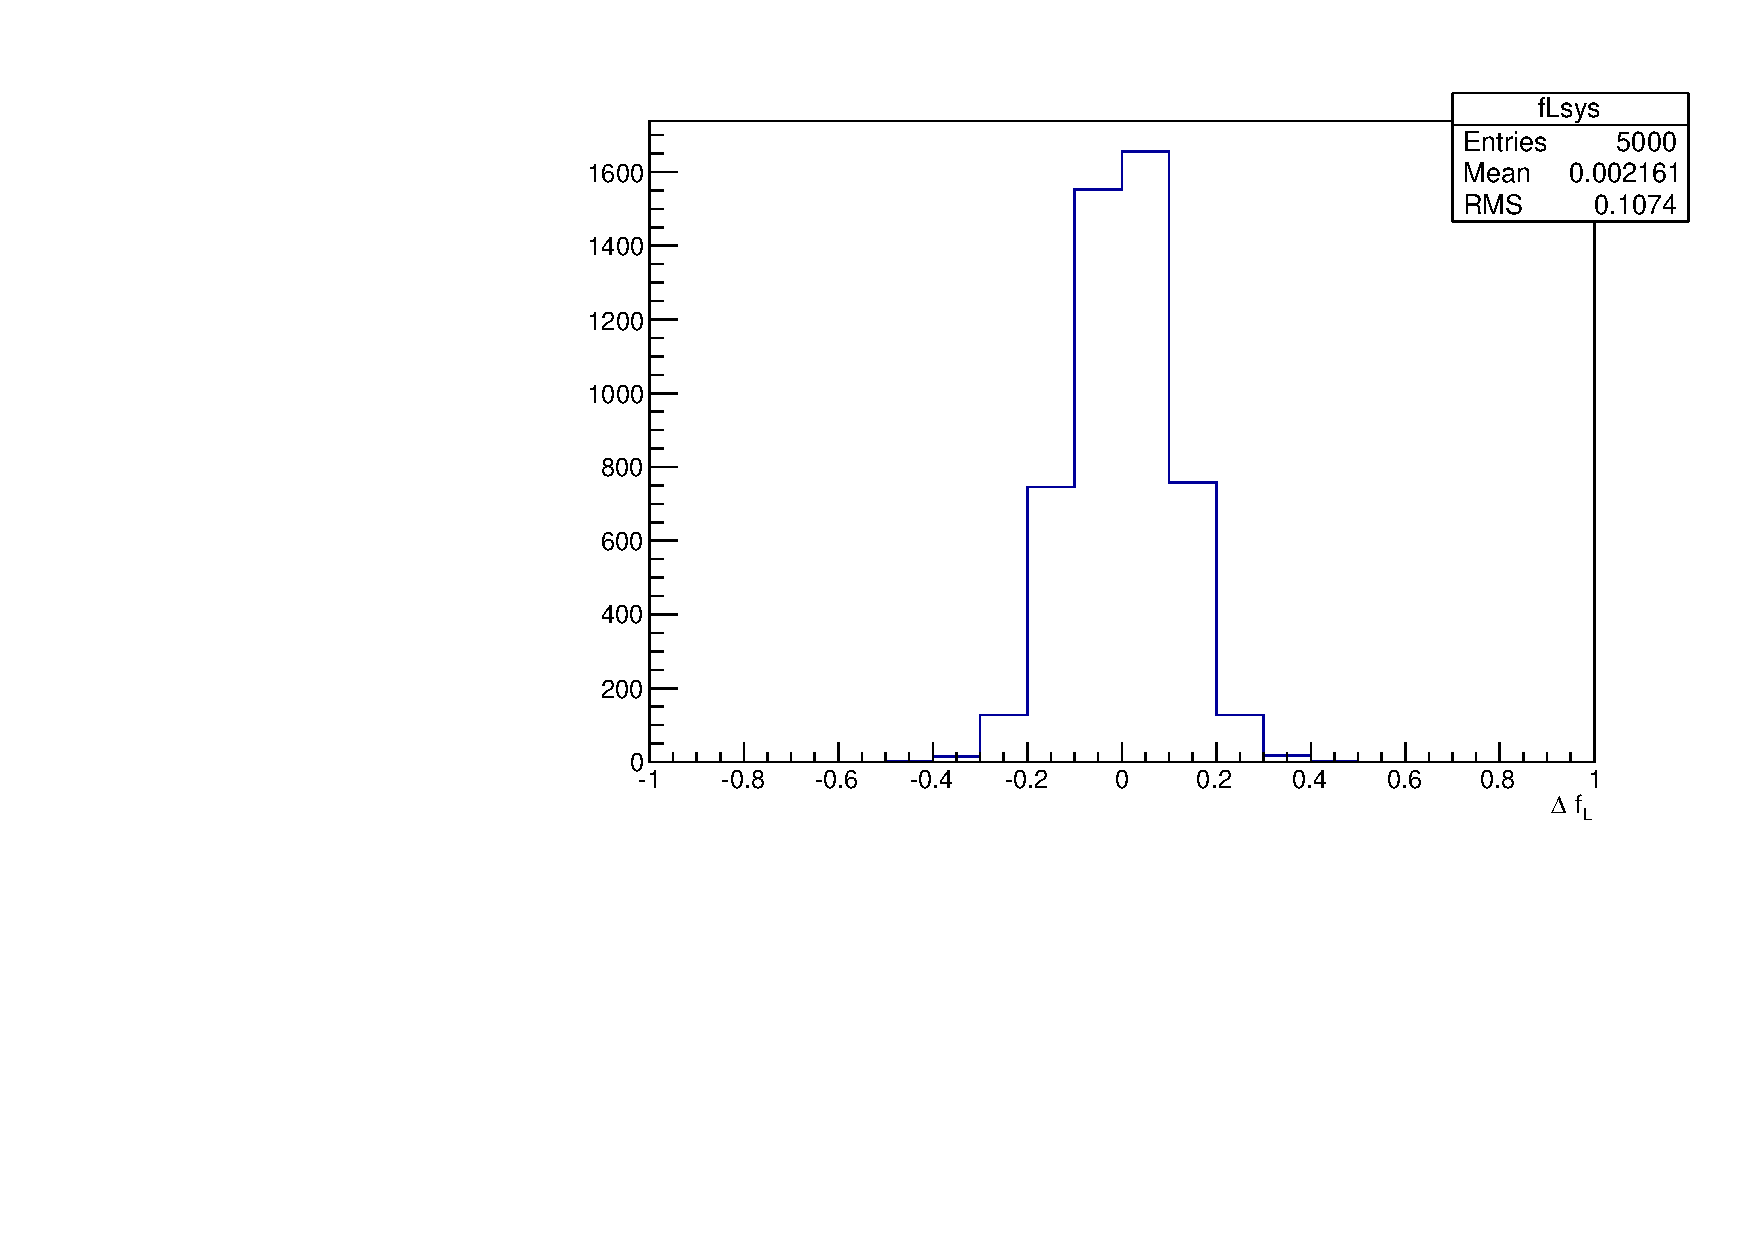
\includegraphics[width=0.45\textwidth]{Lmumu/figs/fLsys_polarisation.pdf}
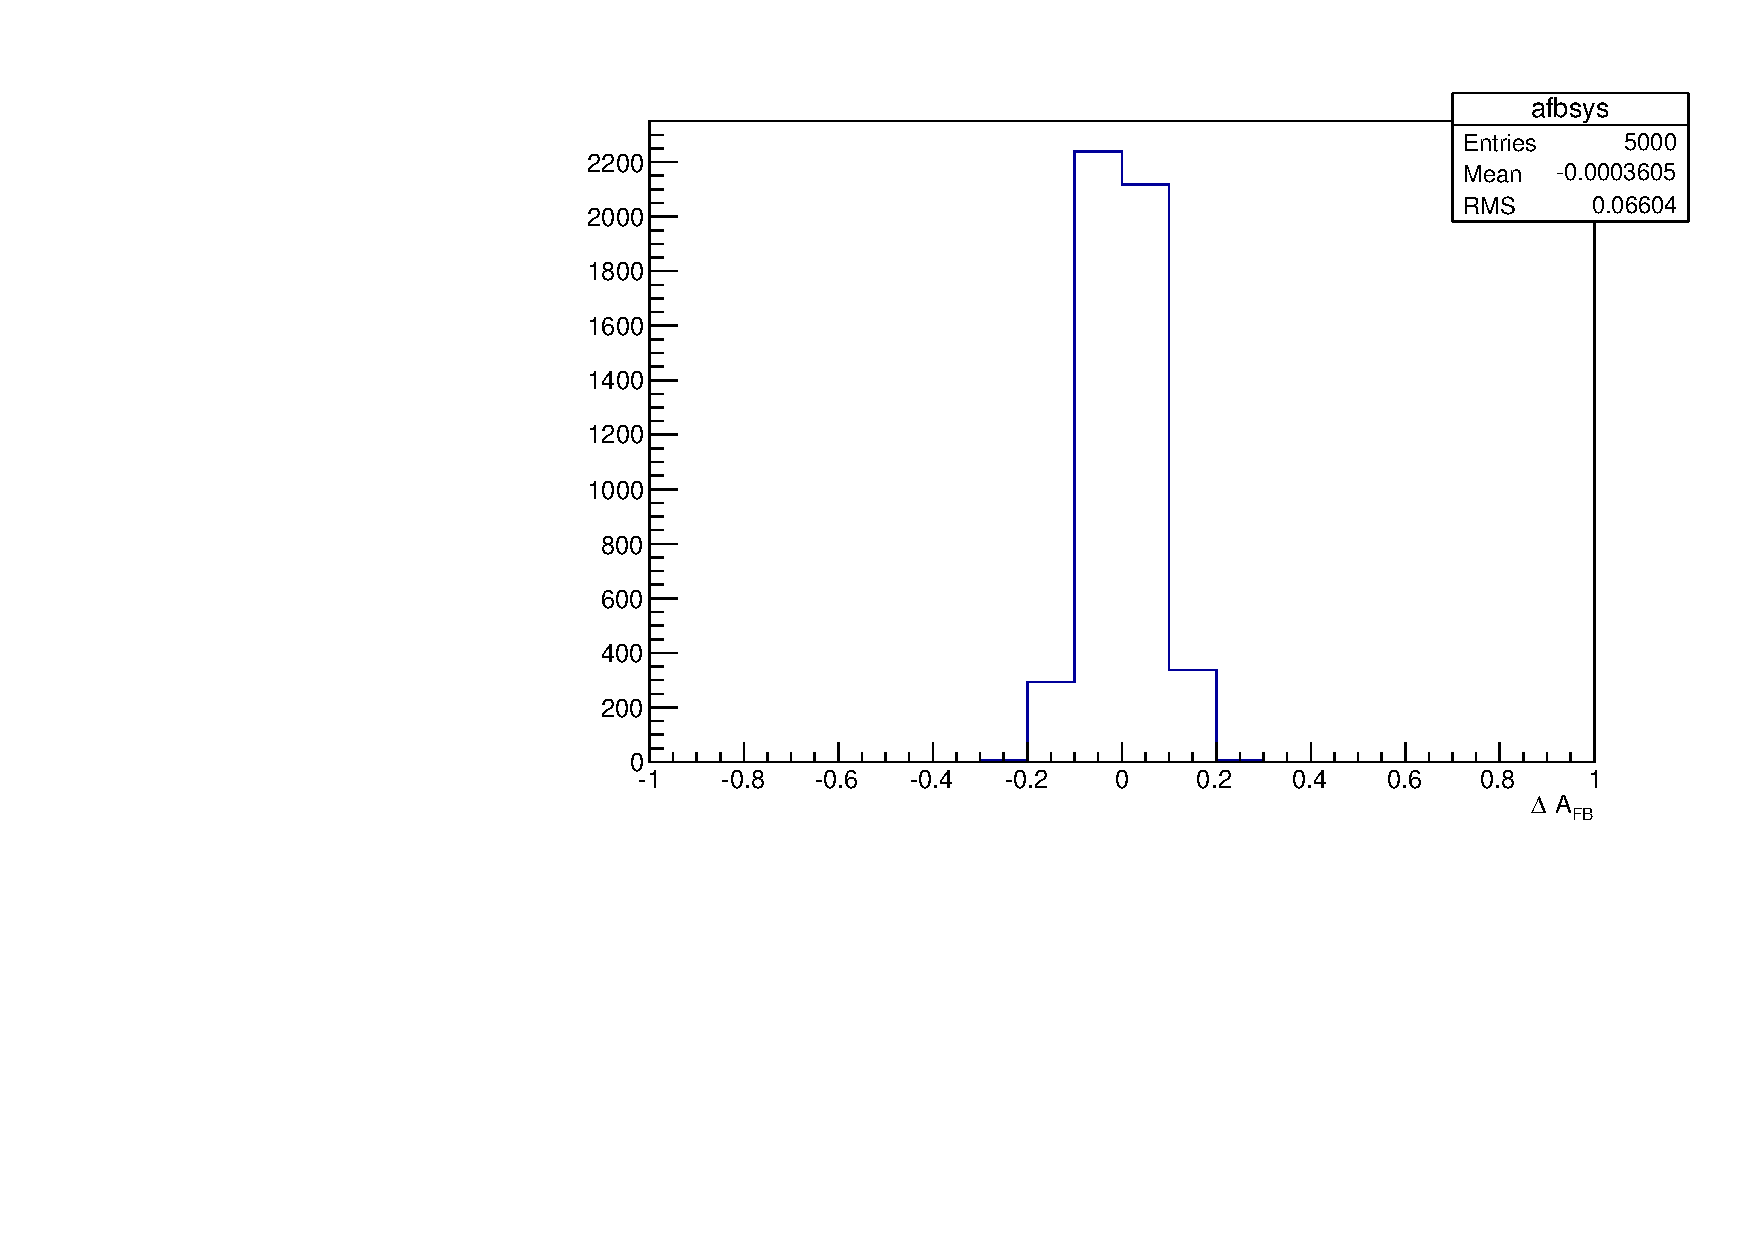
\includegraphics[width=0.45\textwidth]{Lmumu/figs/afbsys_polarisation.pdf}
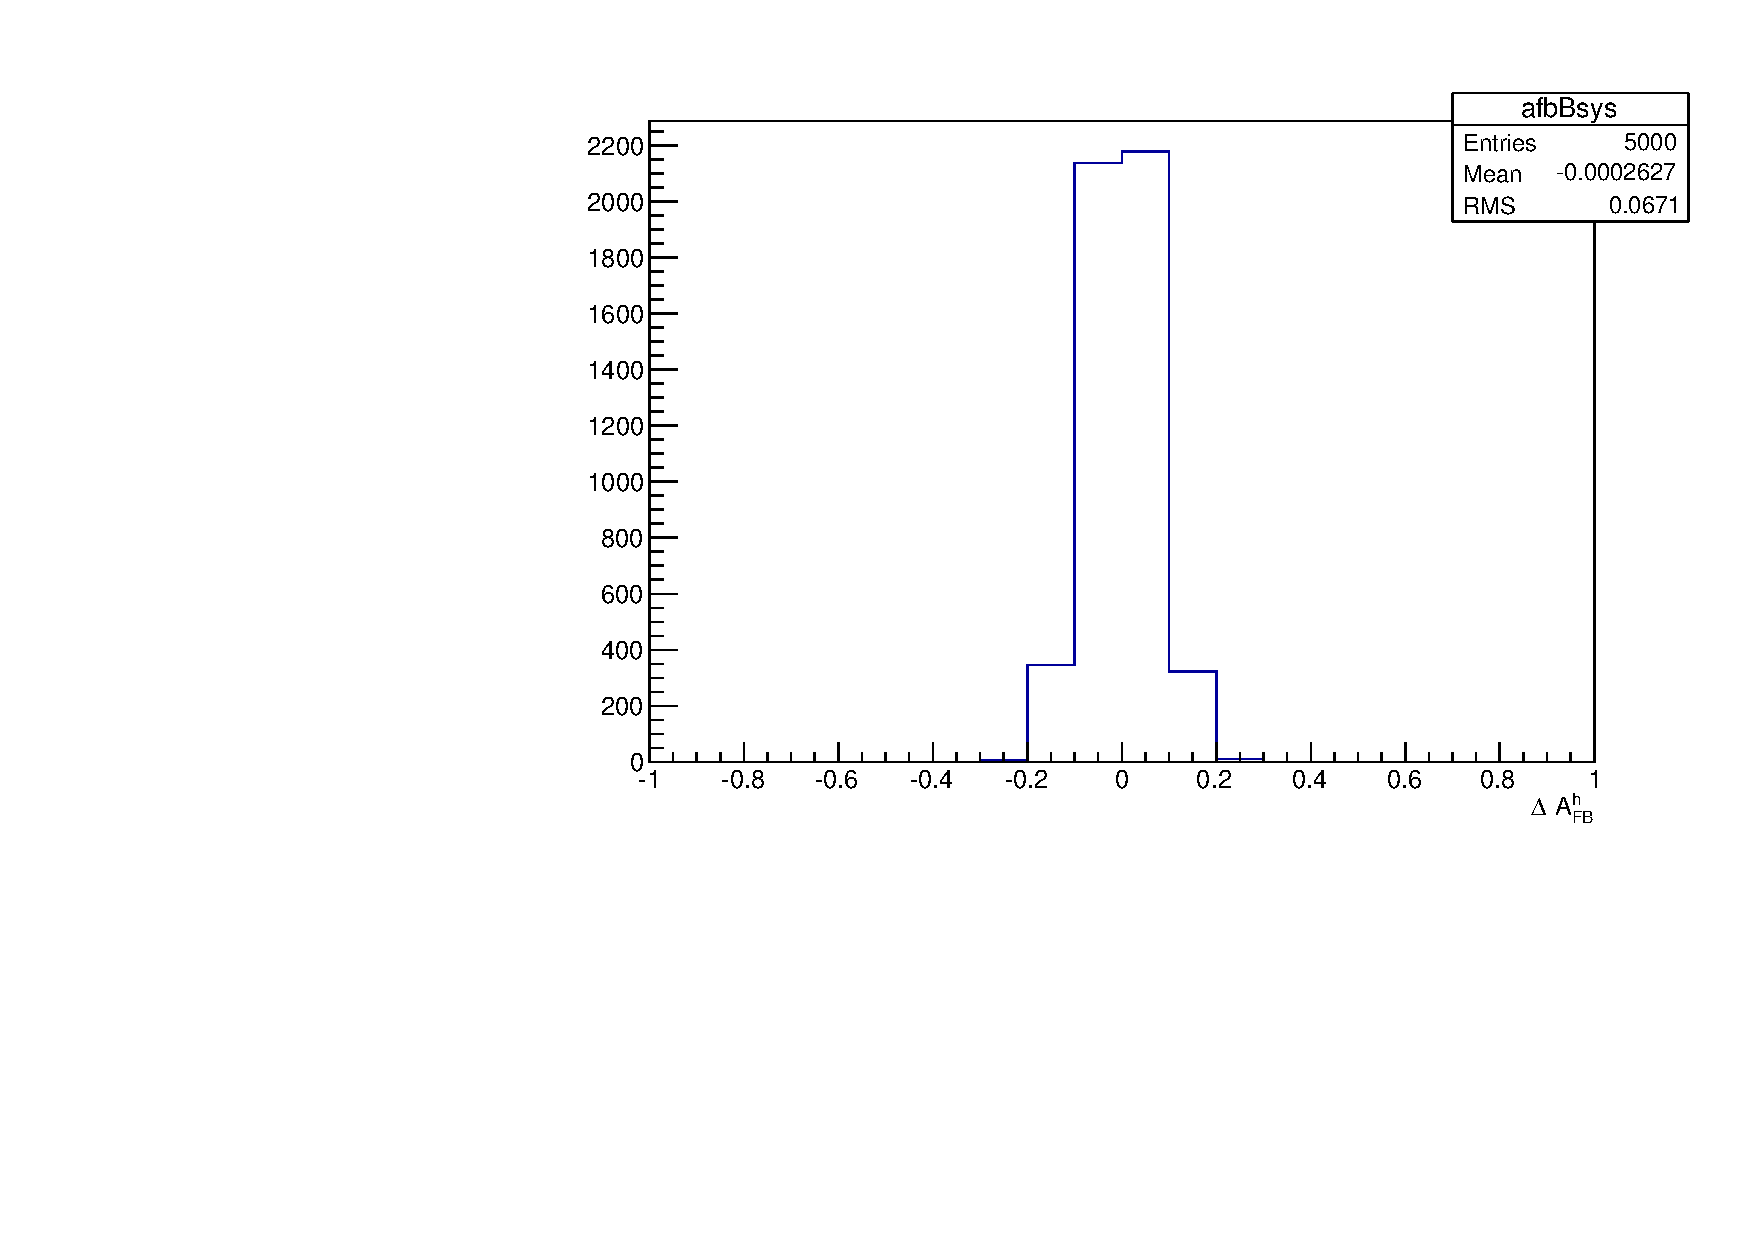
\includegraphics[width=0.45\textwidth]{Lmumu/figs/afbBsys_polarisation.pdf}
\caption{Plots show the absolute difference of the observables' values obtained fitting toy MC generated with polarisation set to $-0.03$ and $+0.15$. From left to right for $f_L$, $A_{FB}^\ell$ and $A_{FB}^h$. }
\label{fig:Afbpolsys}
\end{figure}




\section{$J/\psi$ cross-check}

In order to cross-check our fitting procedure we apply it on $J/\psi$ events, for which we have higer statistics.
To select these events we apply the same selestion ad for the branching fraction (see sec. \ref{sec:selection}) with
the addition of a strong PID cut on the proton ($PID_{p\rightarrow p} > 10$), needed to reduce the
\KS\jpsi background. This is particularly important for the $cosTheta_{\Lambda}$ fit, since 
the \KS events are not distributed in a flat way in this waribale and therefore can bias the fit.
In Fig. \ref{fig:Jpsimass_angular} are reported mass plots after this cut, which can be comparend with
Fig. \ref{fig:totalFit}, and one can see that the \KS background is reduced. After the PID cut we have 0.2\% of \KS
events in down-down events and a fraction compatible with zero in long-long events.

The signal fit model is the same used for the rare case and described in \ref{sec:AngEff},
for the background instead the higher statistics allows to leave more freedom to the fit.
Therefore we use a 2nd order Chebyschev polynomial where the two parameters are fitted directly on upper sideband background.
As for the rare case the background fractions are gaussian-constrained in the fit.

In Figs. \ref{fig:AngFitJpsi}, \ref{fig:AngFitBJpsi} are reported angular fits for the \jpsi channel. The values of the observables extracted are $A_{FB}^\ell = -0.002^{+0.011}_{-0.011}$, $A_{FB}^h = -0.402^{+0.010}_{-0.009}$ and $f_{L} = 0.485^{+0.019}_{-0.020}$, where the errors are 1D Feldman cousins (for $A_{FB}^\ell$ and $f_L$ the parameters are taken into account one at a time while the other is considered a nuisance).

\begin{figure}
\centering
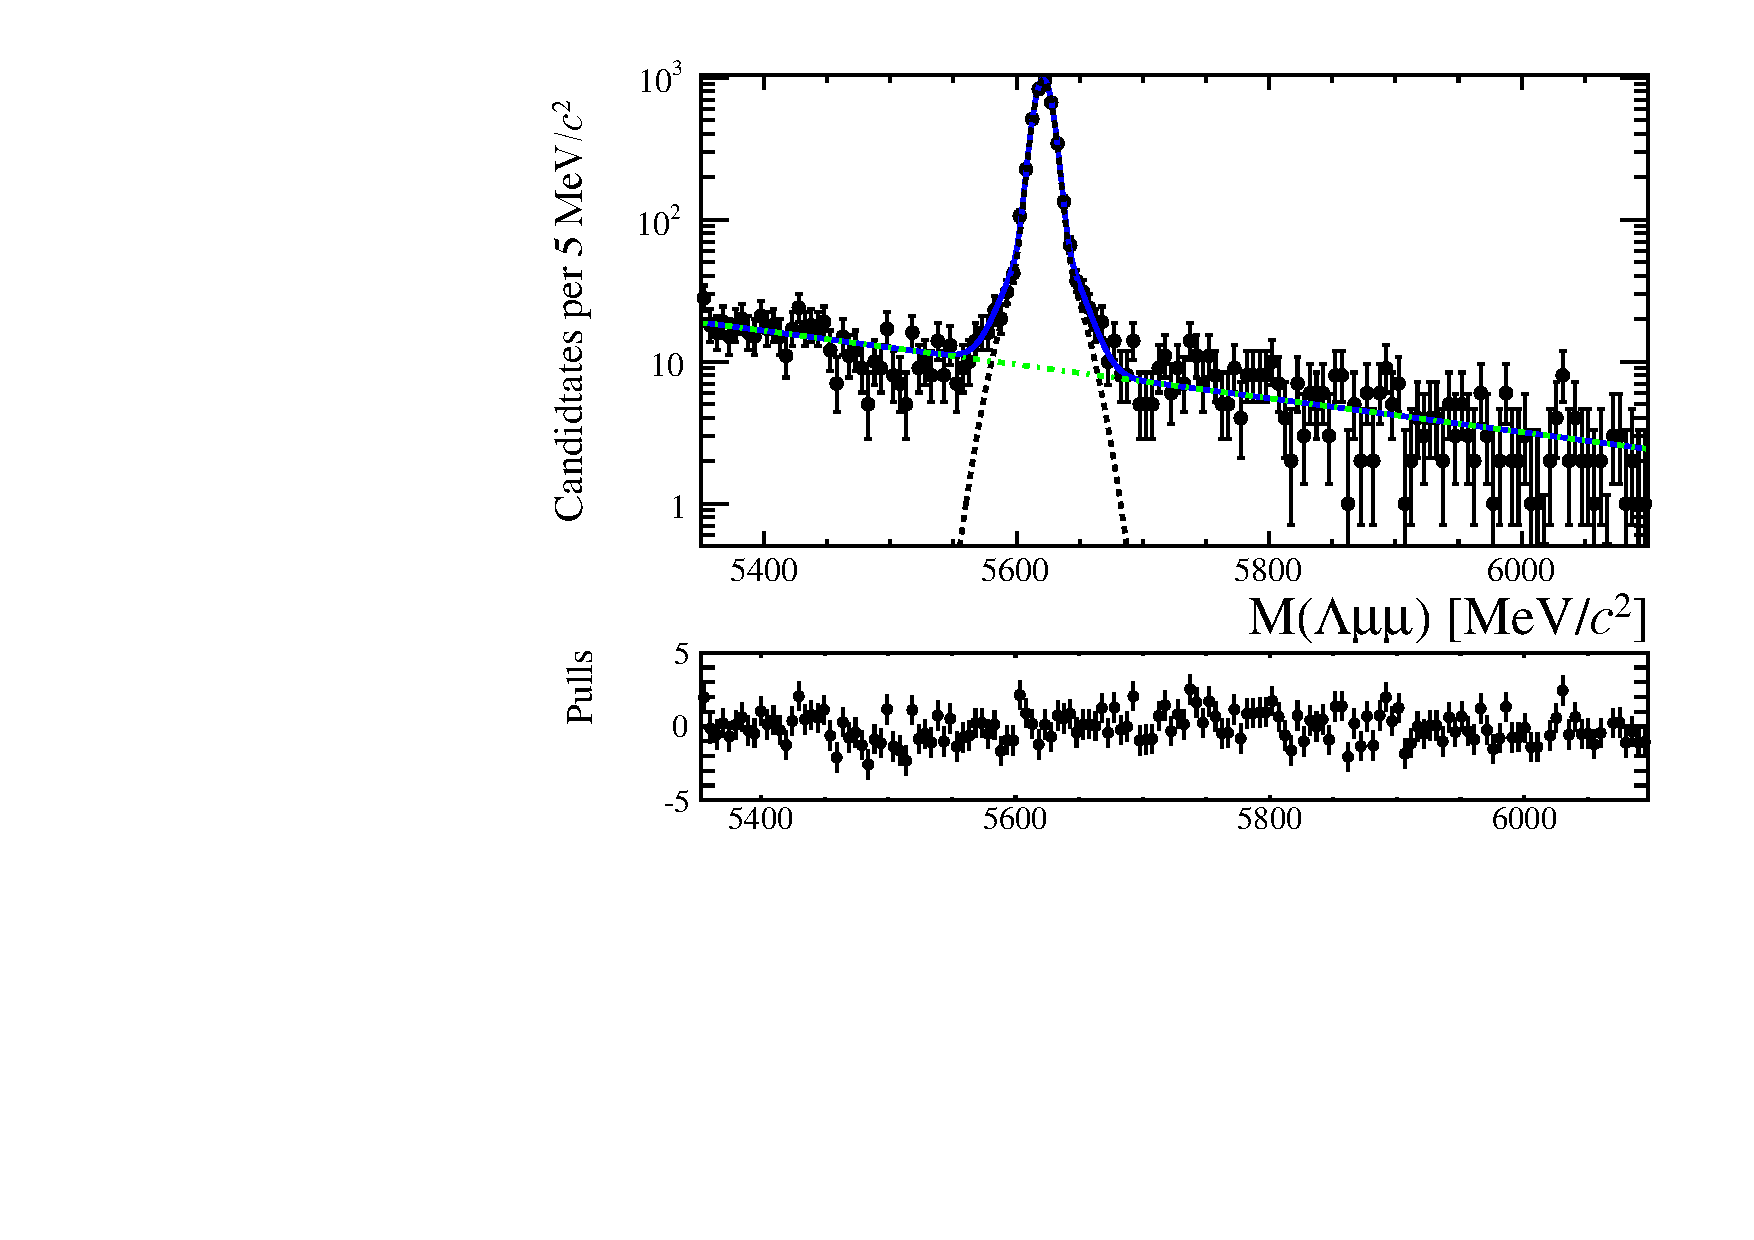
\includegraphics[width=0.45\textwidth]{Lmumu/figs/Jpsi_default_LL_log_fitAndRes.pdf}
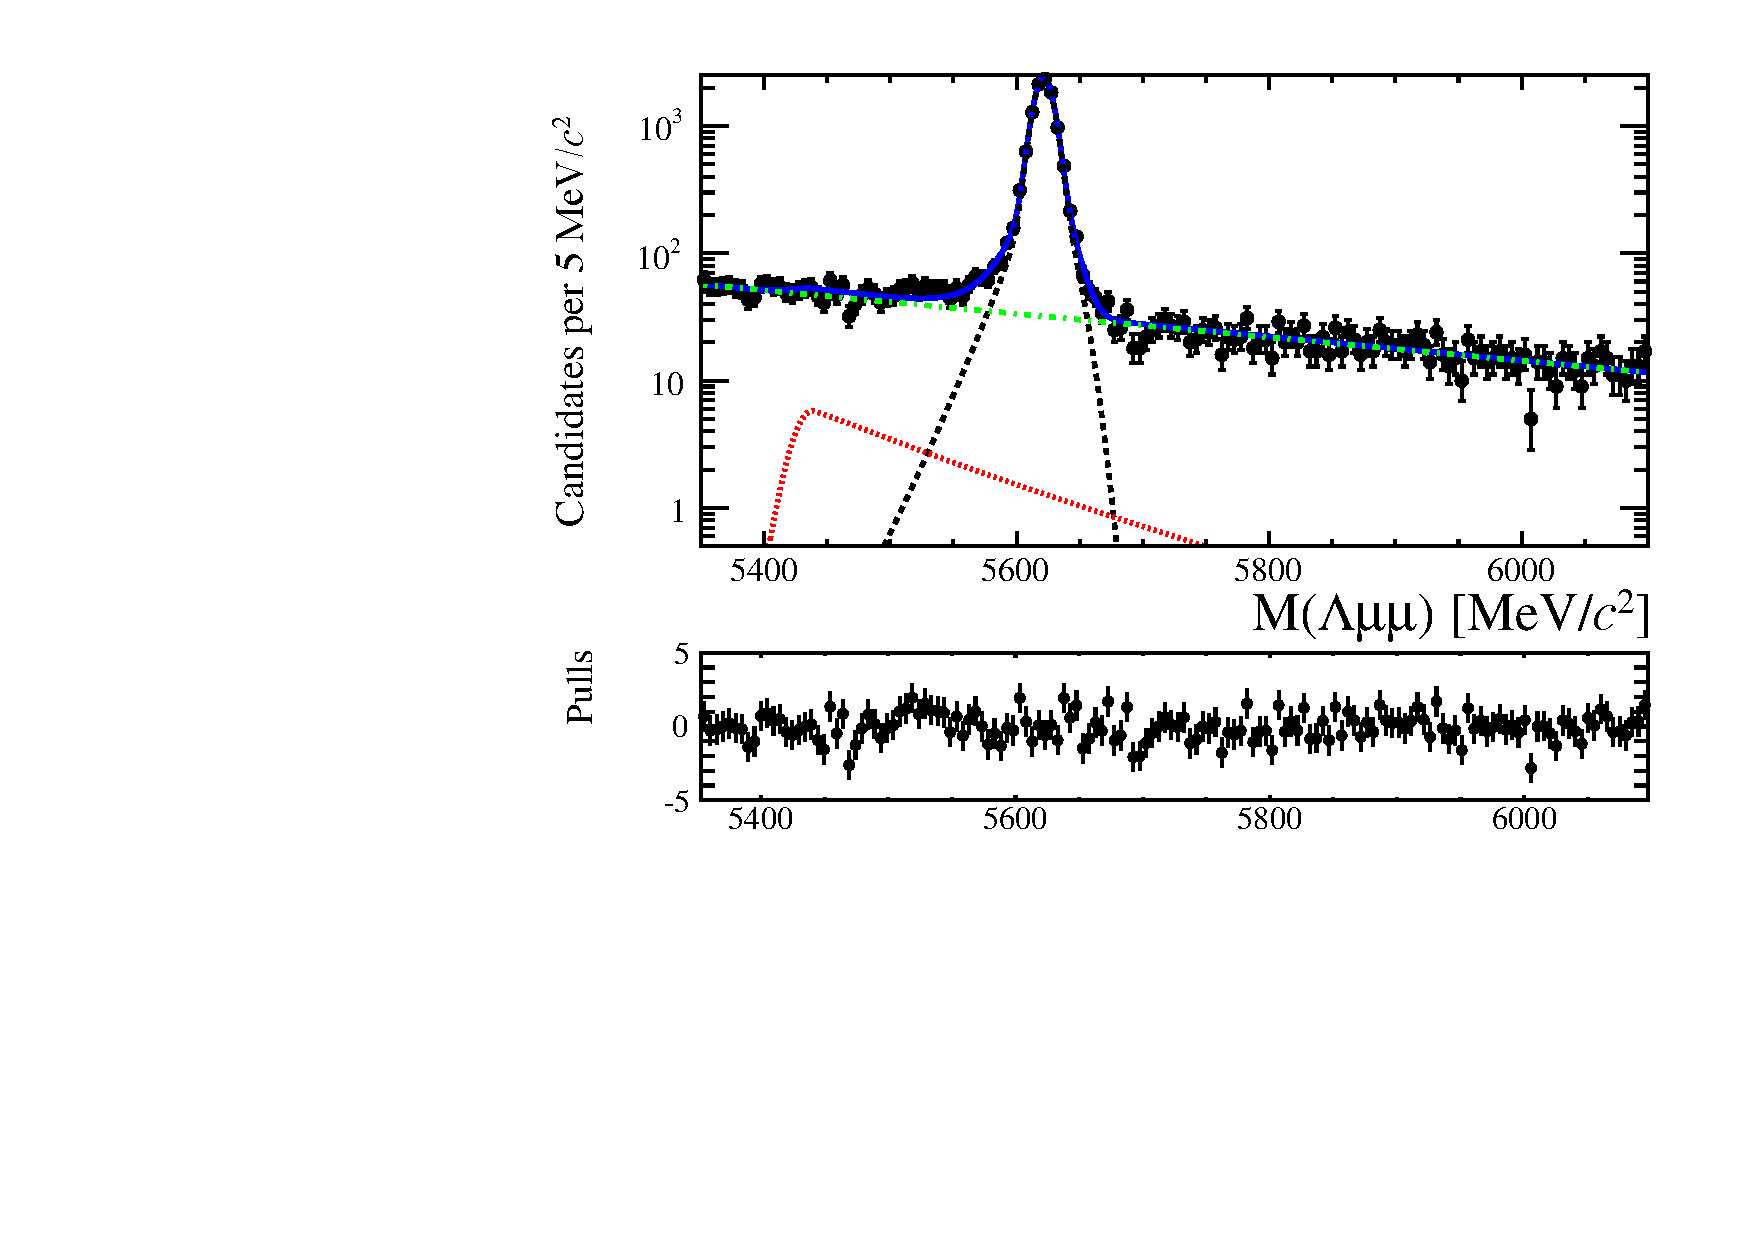
\includegraphics[width=0.45\textwidth]{Lmumu/figs/Jpsi_default_DD_log_fitAndRes.pdf}
\caption{Invariant mass distribution of $\Lb\ra\jpsi\Lz$ and residuals of the fit for long-long (left) and down-down (right) events.
The histogram shows data as in Fig.\ref{fig:totalFit} with an extra proton PID cut to remove \KS background.}
\label{fig:Jpsimass_angular}
\end{figure}
%

\begin{figure}[h]
\centering
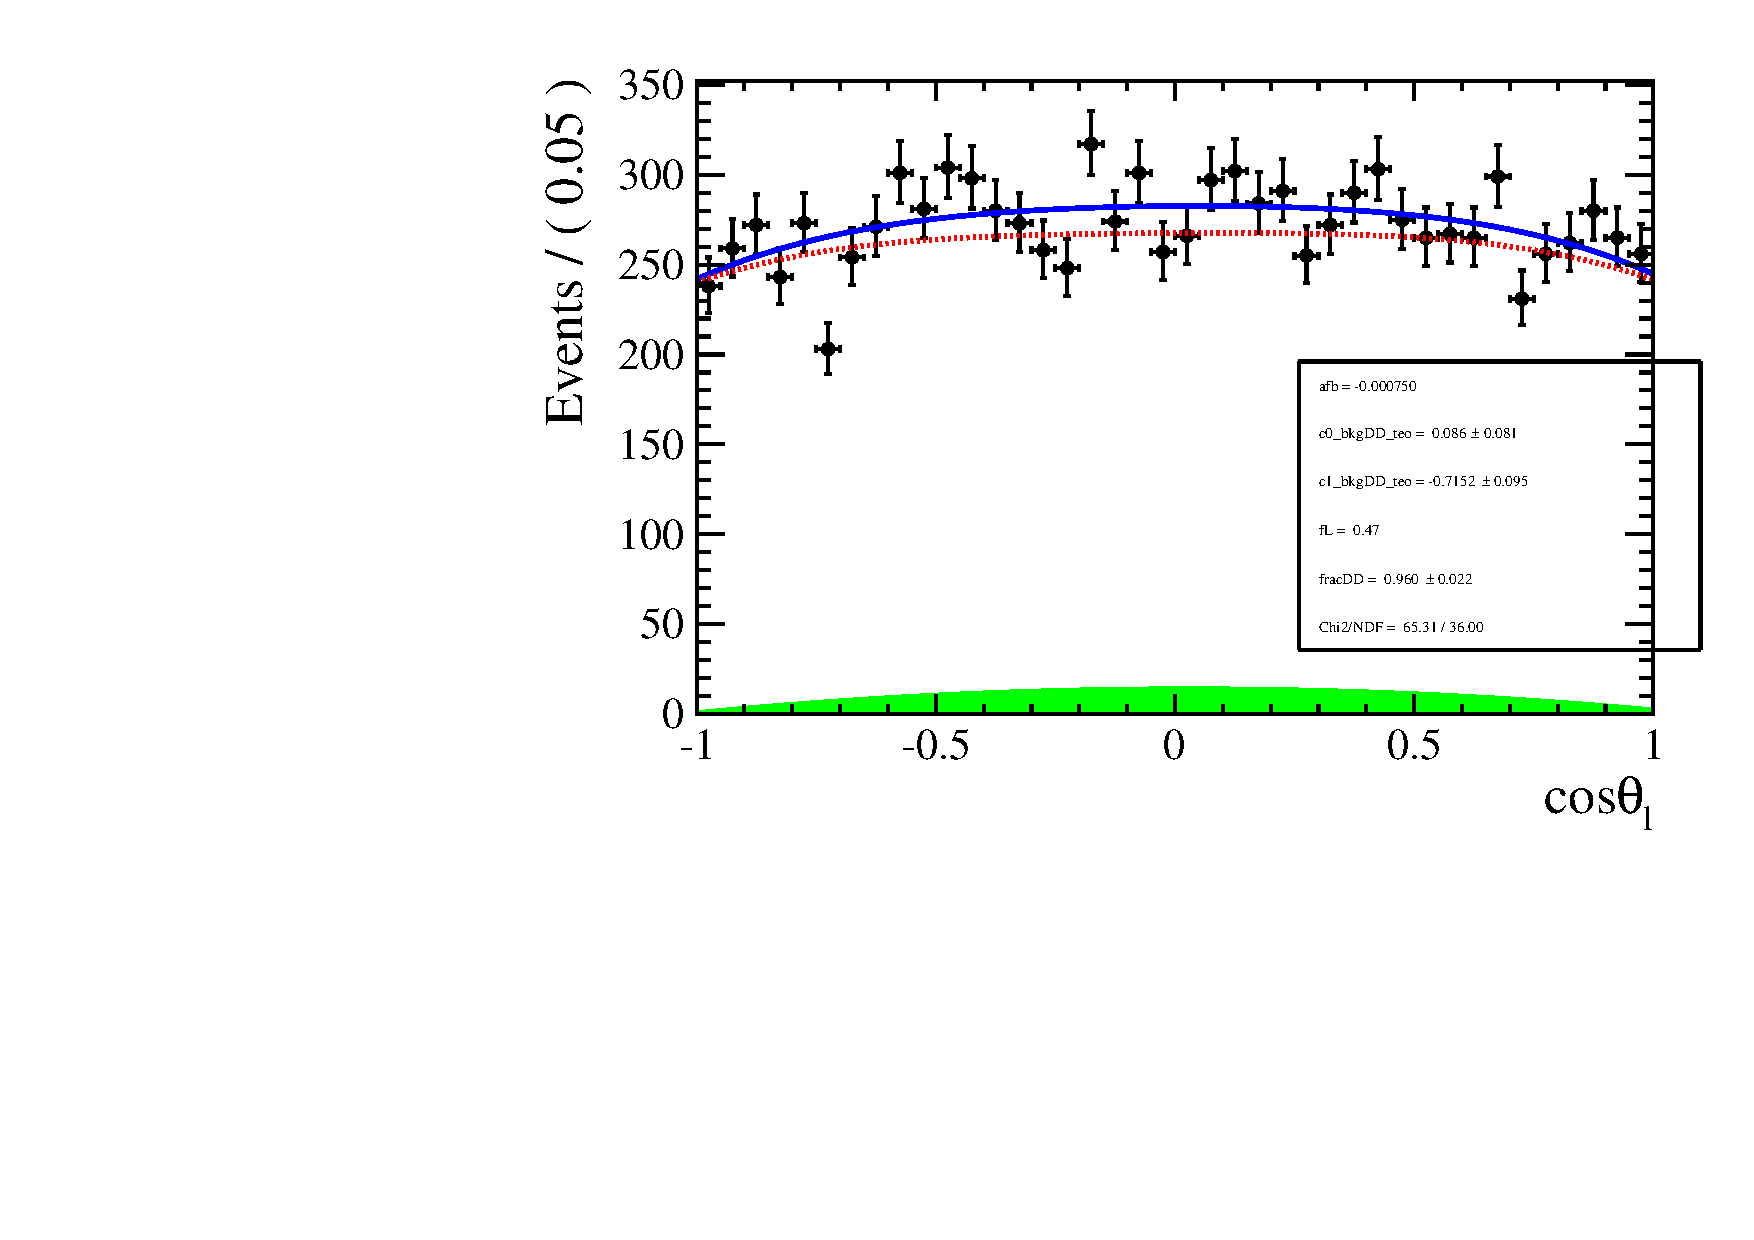
\includegraphics[width=0.45\textwidth]{Lmumu/figs/AngularDistribs/Fitted/Afb_DD_jpsi.pdf}
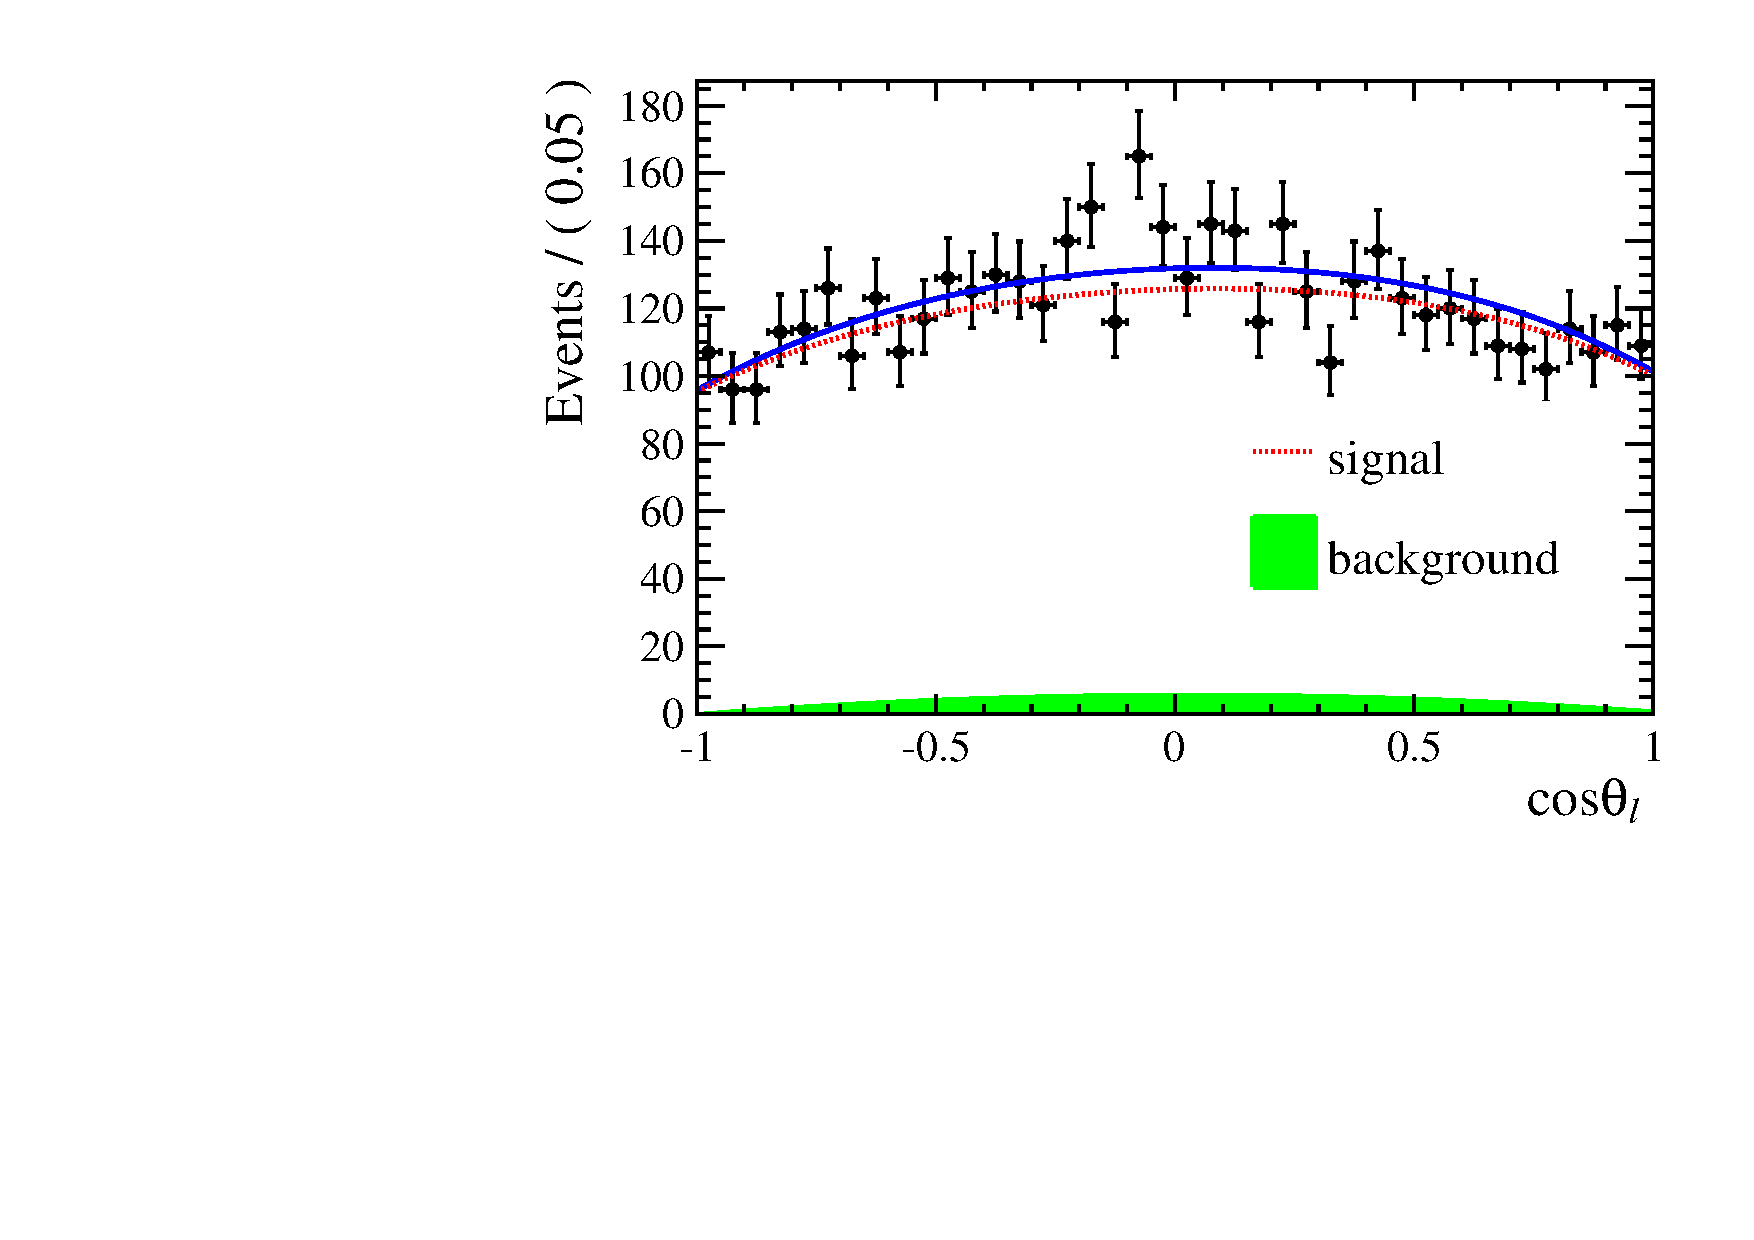
\includegraphics[width=0.45\textwidth]{Lmumu/figs/AngularDistribs/Fitted/Afb_LL_jpsi.pdf}
\caption{Fitted angular distribution as a function of $\cos\theta_\ell$ for down-down (left) and long-long (right) events for $J/\psi$ events.  }
\label{fig:AngFitJpsi}
\end{figure}

\begin{figure}[h]
\centering
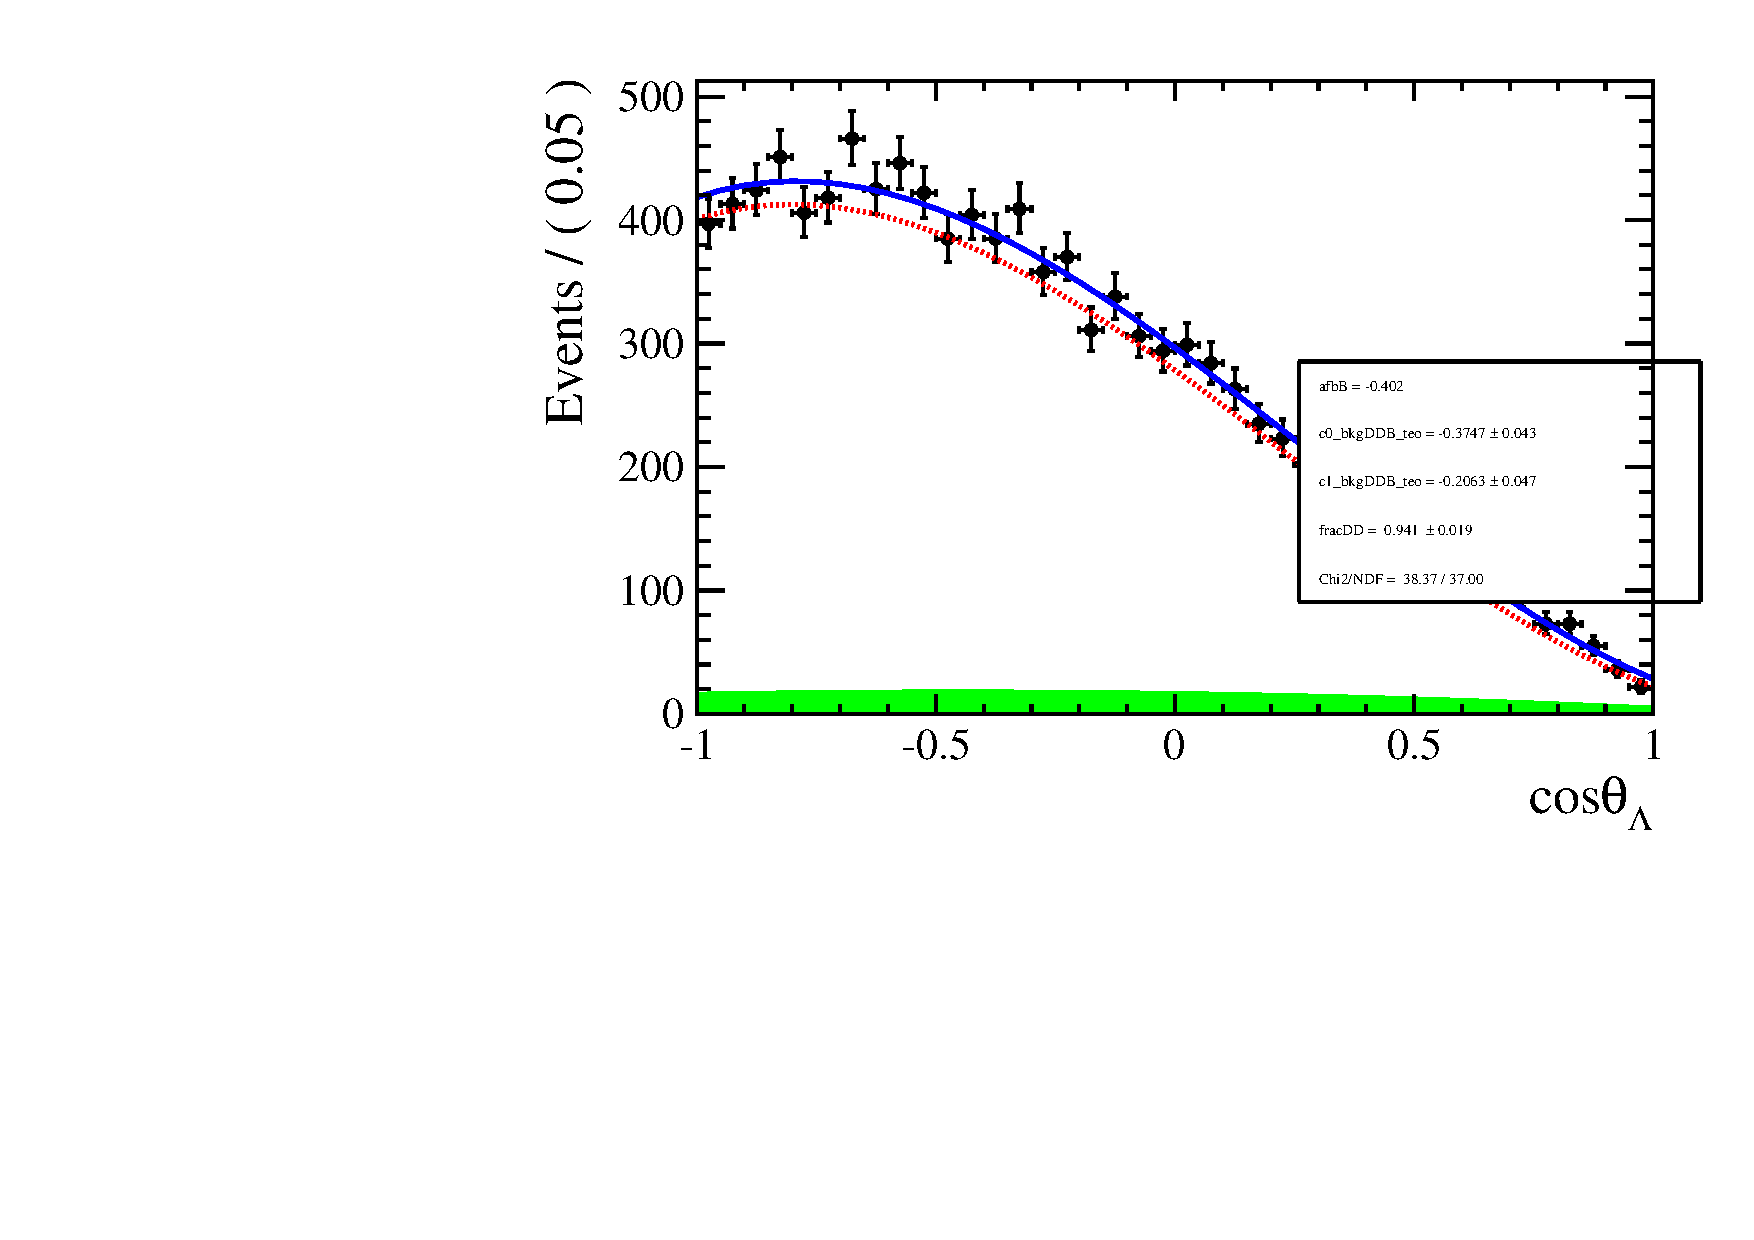
\includegraphics[width=0.45\textwidth]{Lmumu/figs/AngularDistribs/Fitted/AfbB_DD_jpsi.pdf}
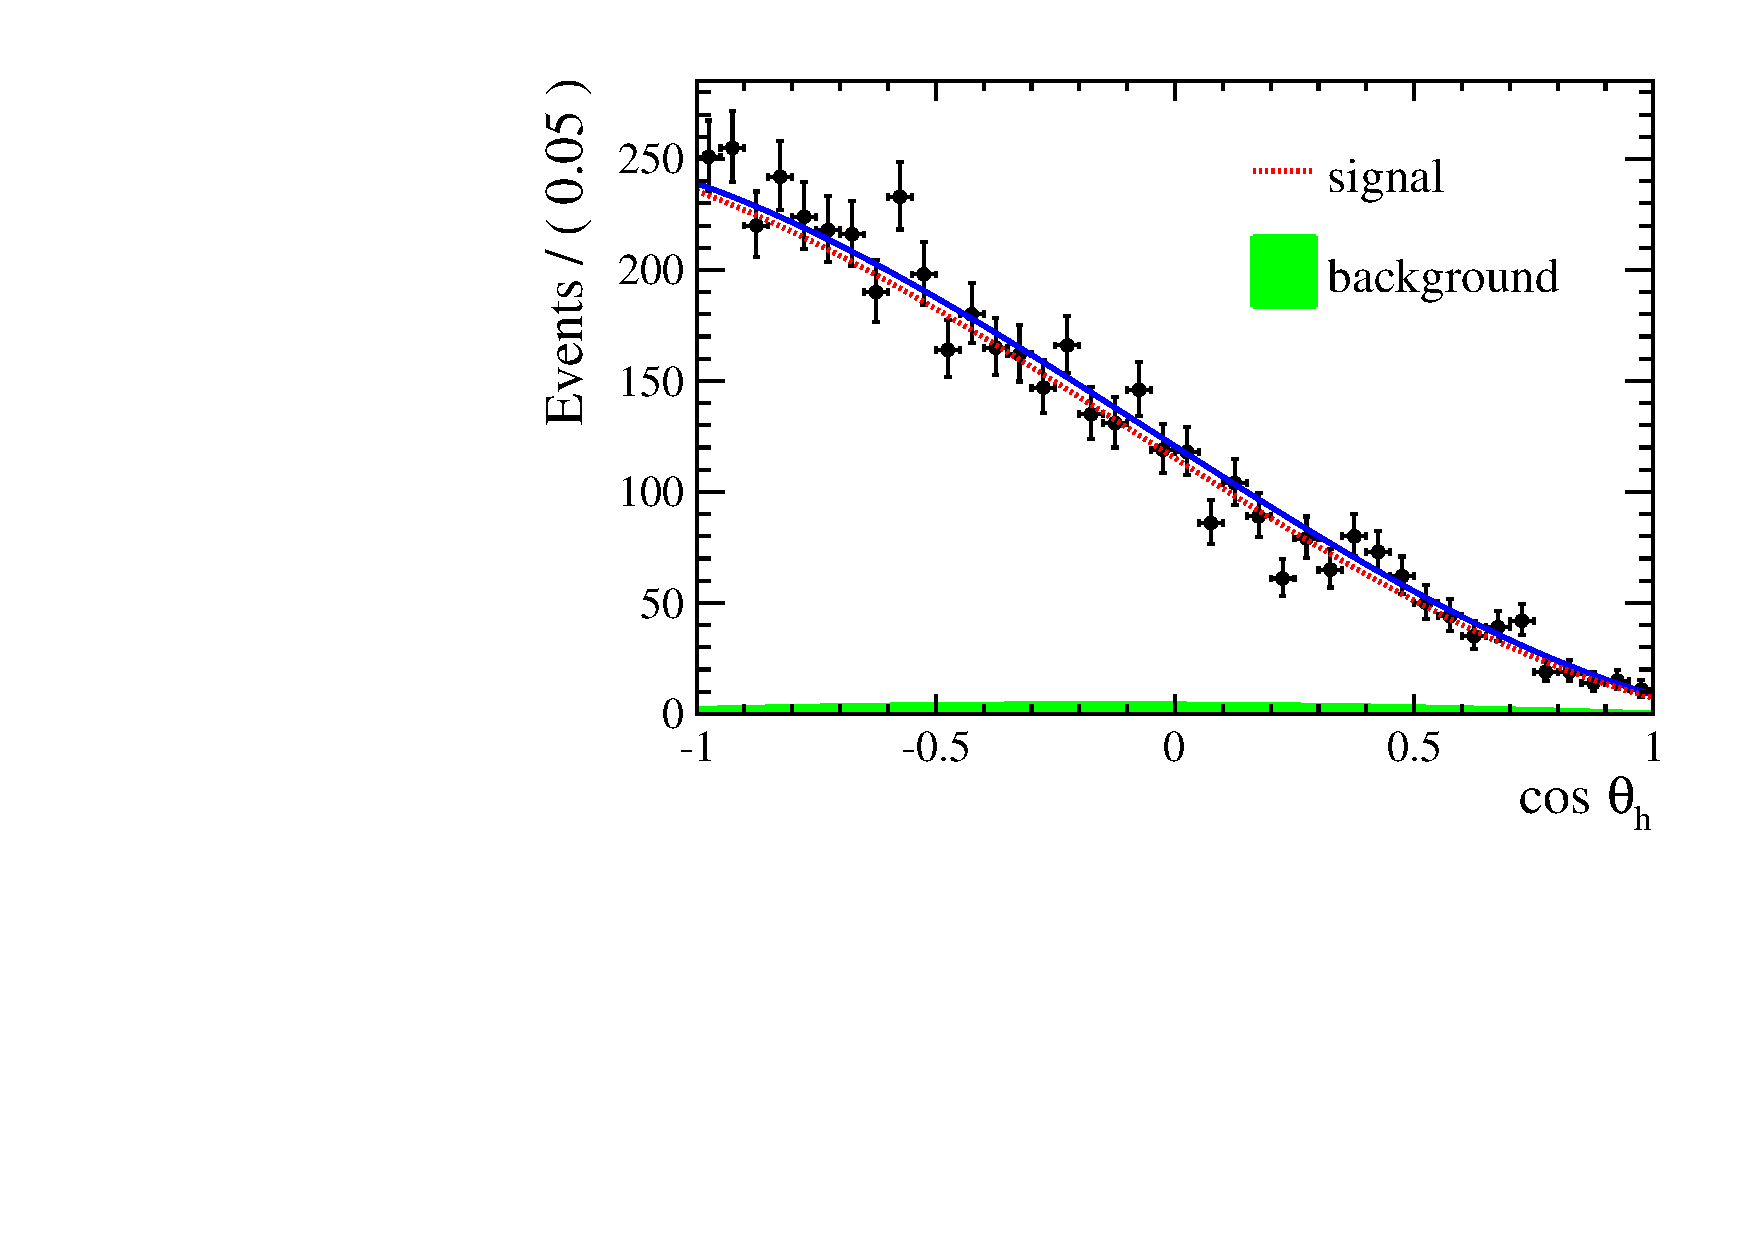
\includegraphics[width=0.45\textwidth]{Lmumu/figs/AngularDistribs/Fitted/AfbB_LL_jpsi.pdf}
\caption{Fitted angular distribution as a function of $\cos\theta_\Lambda$ for down-down (left) and long-long (right) events for $J/\psi$ events.  }
\label{fig:AngFitBJpsi}
\end{figure}







\section{Results}

In Figs. \ref{fig:AngFit} and \ref{fig:AngFitB} are reported angular fits for the 15-20 $GeV^2/c^2$ \qsq bin, fits in all other \qsq bins
are reported in appendix \ref{app:AngRes}. 
The LL and DD distributions are fitted simultaneously and therefore we only have two free parameters
in the fit, $f_L$ and $A_{FB}^\ell$, for the lepton side and one, $A_{FB}^h$, for the hadron one.

In tables \ref{tab:afblresults} and \ref{tab:afbhresults} are reported values of $A_{FB}^l$, $A_{FB}^h$ and $f_L$
in the same \qsq binning used for the branching fraction measurement. 
The statistical errors shown are asymmetric 68\% CL intervals, obtained using the Feldman-Cousins method.
For the $\cos\theta_{ell}$ case we report statistical errors as 2D condifence regions shown in Fig.\ref{fig:contours}.
Systematic errors are square root sum of the sources considered.

\begin{figure}[h]
\centering
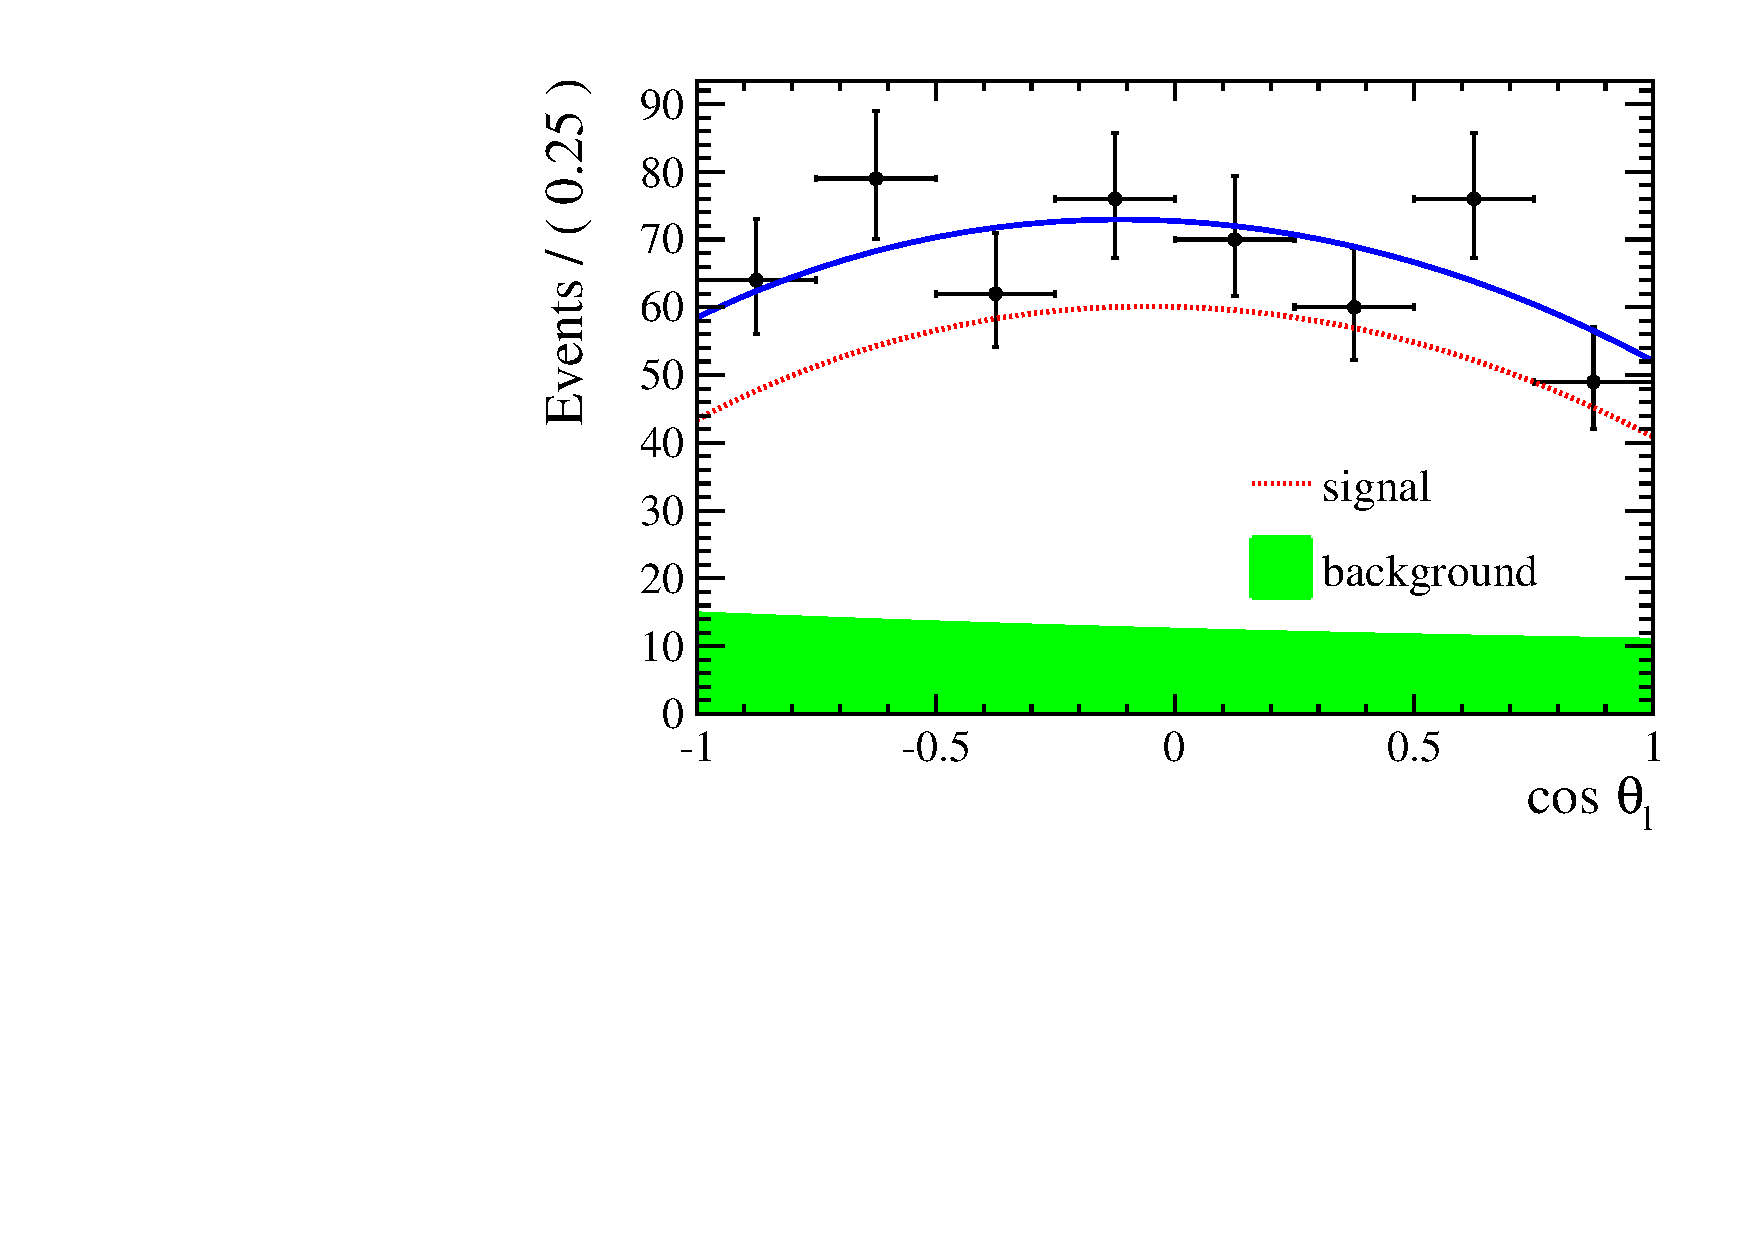
\includegraphics[width=0.45\textwidth]{Lmumu/figs/AngularDistribs/Fitted/Afb_DD_q2_1500_2000.pdf}
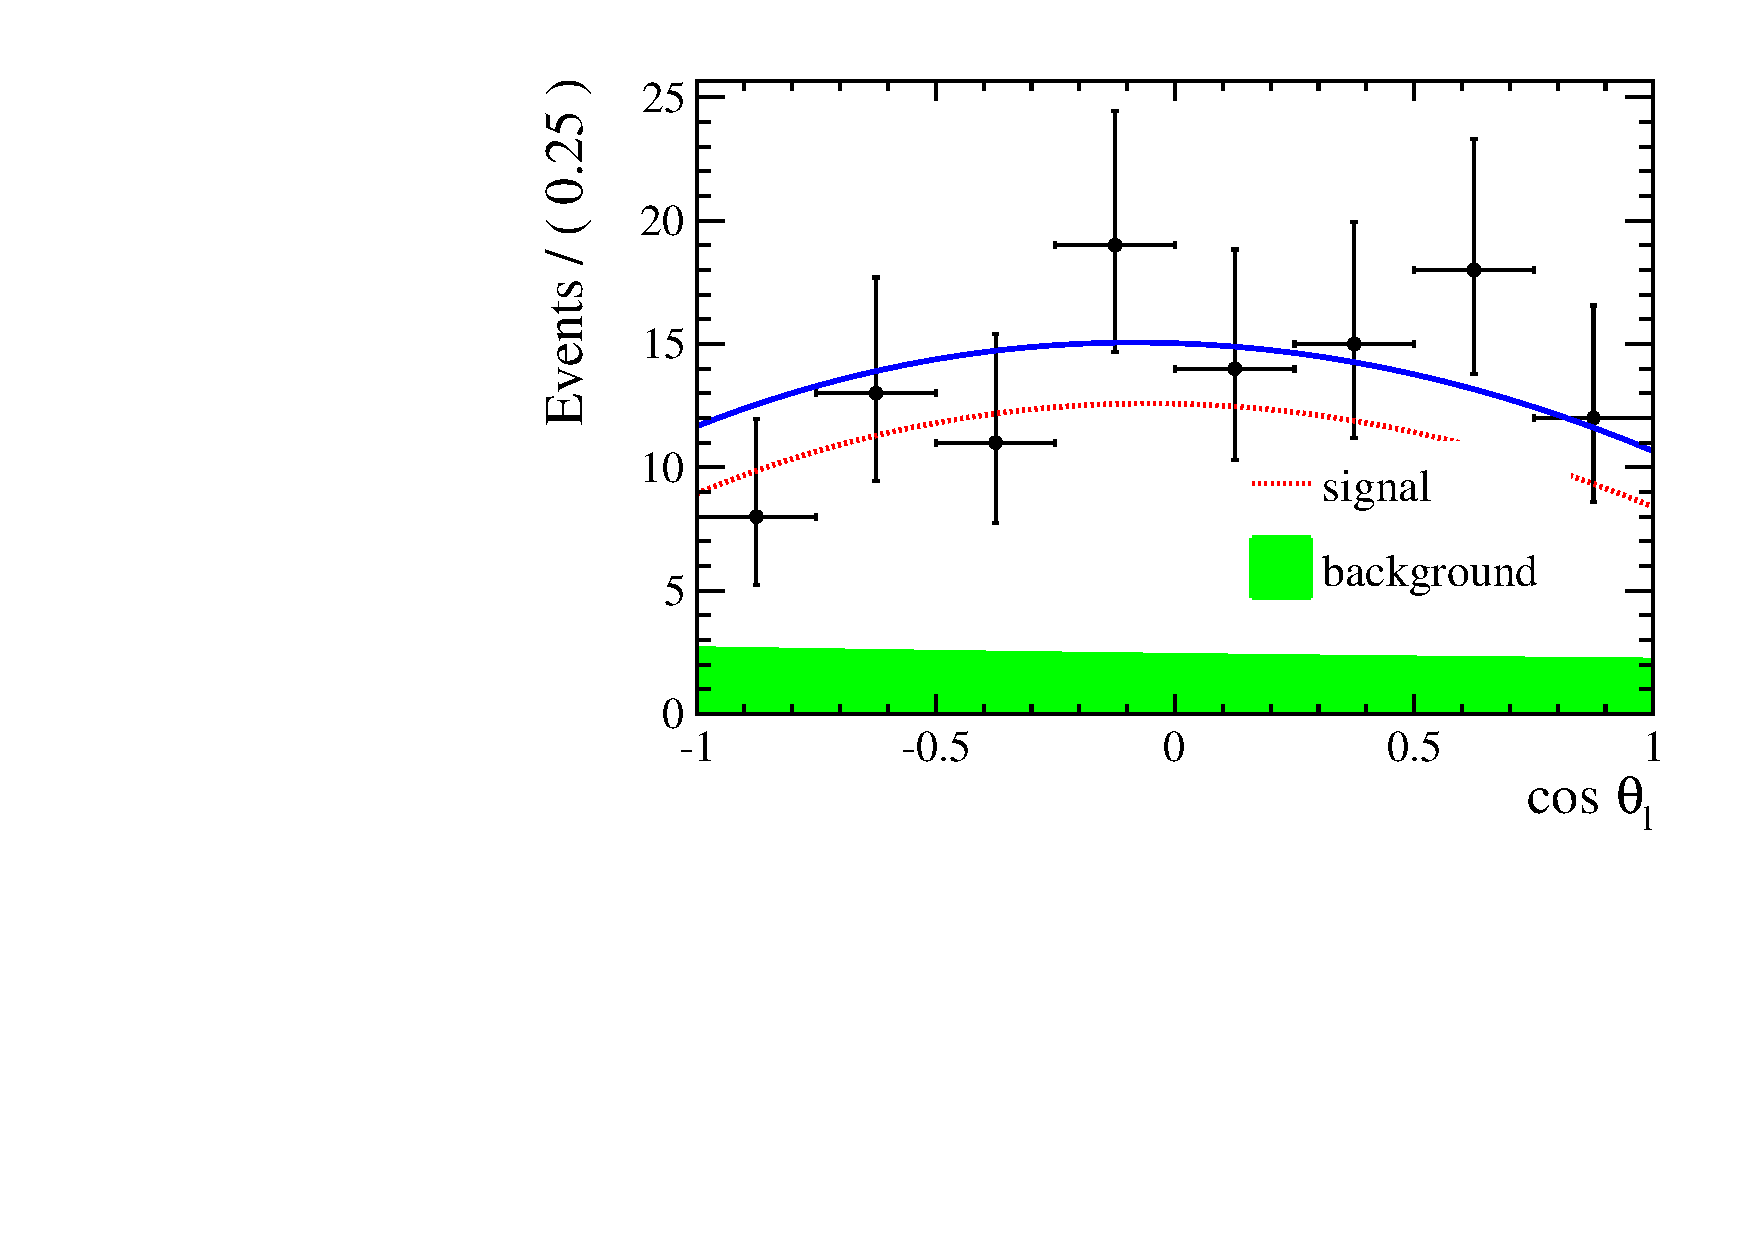
\includegraphics[width=0.45\textwidth]{Lmumu/figs/AngularDistribs/Fitted/Afb_LL_q2_1500_2000.pdf}
\caption{Fitted angular distribution as a function of $\cos\theta_\ell$ for down-down (left) and long-long (right) events in the 15-20$GeV^2/c^2$ \qsq bin.  }
\label{fig:AngFit}
\end{figure}

\begin{figure}[h]
\centering
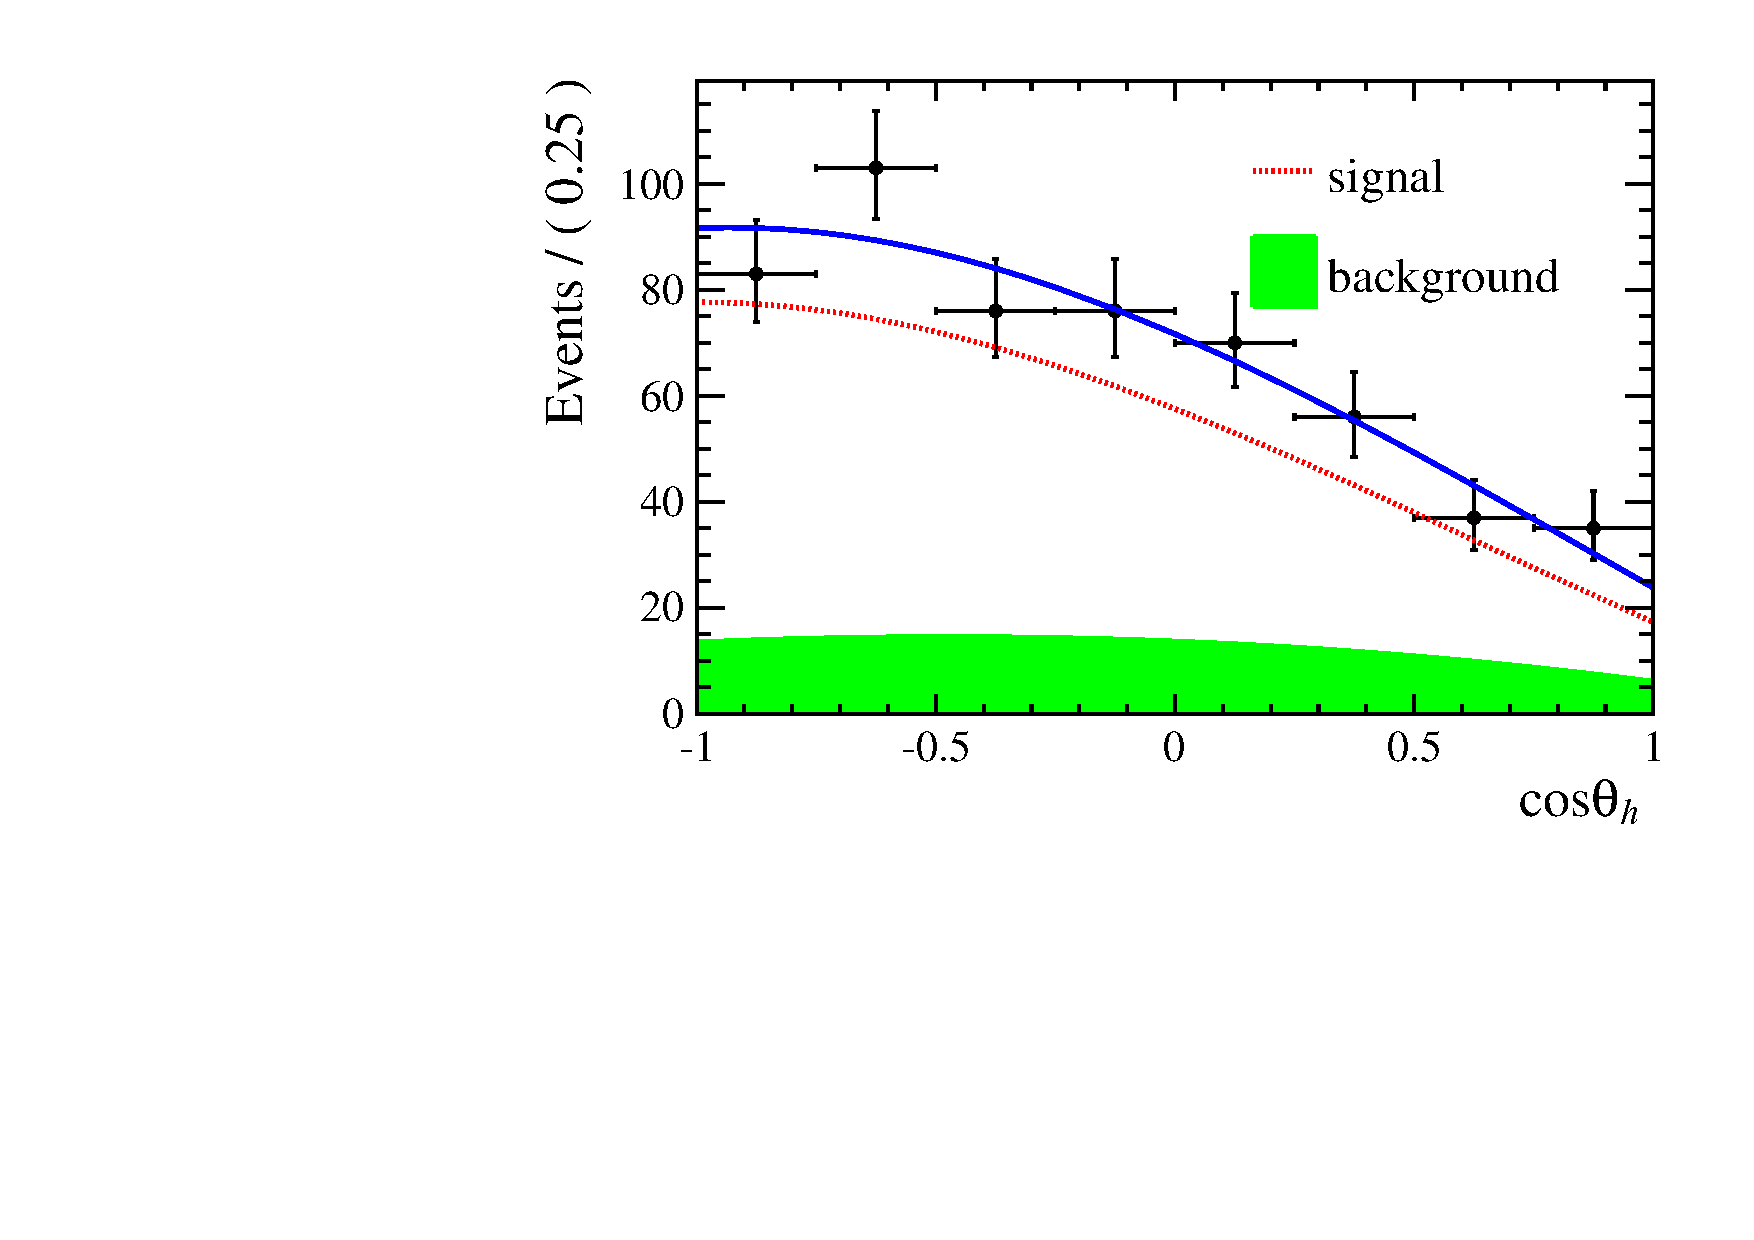
\includegraphics[width=0.45\textwidth]{Lmumu/figs/AngularDistribs/Fitted/AfbB_DD_q2_1500_2000.pdf}
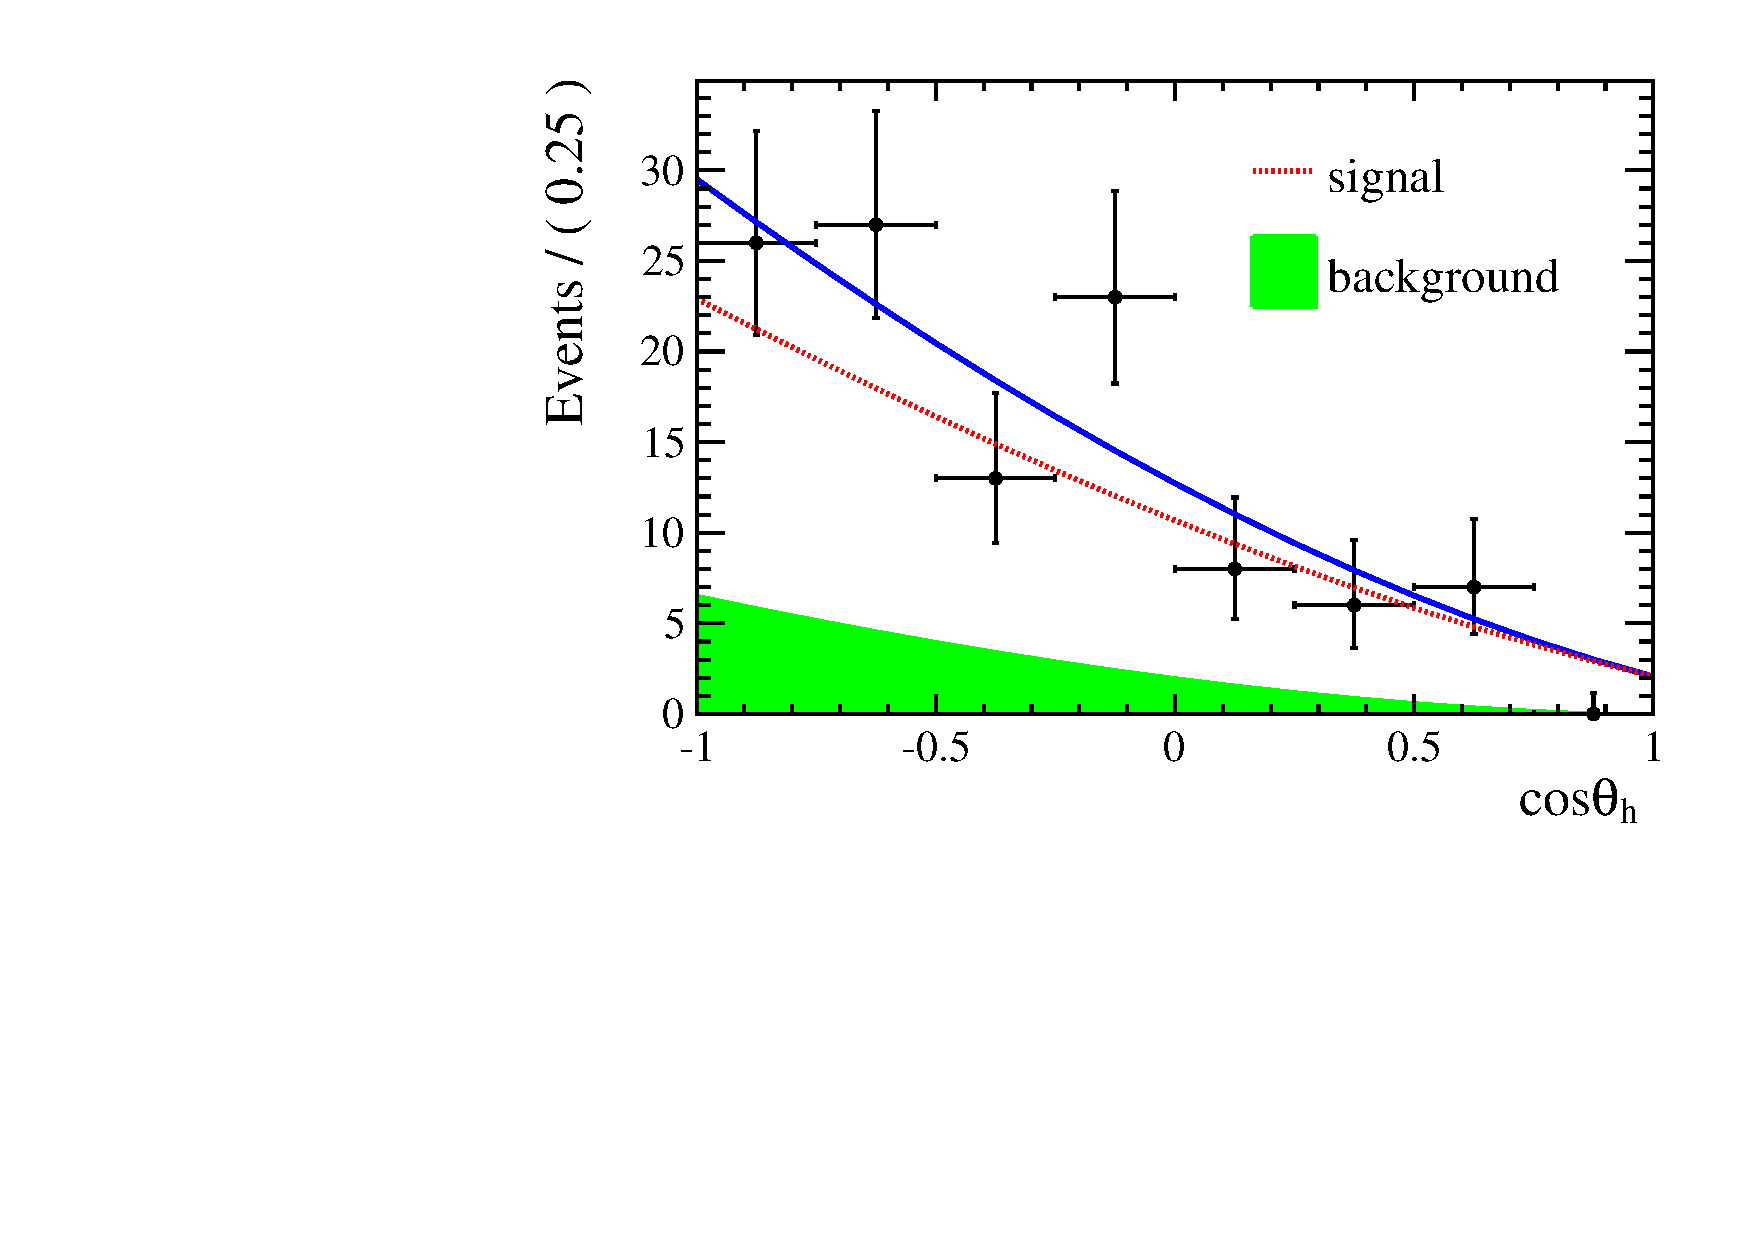
\includegraphics[width=0.45\textwidth]{Lmumu/figs/AngularDistribs/Fitted/AfbB_LL_q2_1500_2000.pdf}
\caption{Fitted angular distribution as a function of $\cos\theta_\Lambda$ for down-down (left) and long-long (right) events in the 15-20$GeV^2/c^2$ \qsq bin.  }
\label{fig:AngFitB}
\end{figure}



\begin{table}[h!]
\centering
\begin{tabular}{c|c|c}
 \qsq bin   &            $A_{FB}^\ell$                                            &       $f_{L}$                     \\ \hline
0.1  - 2.0  & $0.3710_{-0.475}^{+0.370}    \text{(stat)} \pm  0.034 \text{(sys)}$  & $0.559_{-0.559}^{+0.231}  \text{(stat)} \pm 0.083 \text{(sys)}$ \\
11.0 - 12.5 & $0.0083_{-0.1807}^{+0.1944}  \text{(stat)} \pm  0.056 \text{(sys)}$  & $0.398_{-0.359}^{+0.366}  \text{(stat)} \pm 0.058 \text{(sys)}$ \\
15.0 - 16.0 & $-0.1027_{-0.1649}^{+0.1821} \text{(stat)} \pm  0.034 \text{(sys)}$  & $0.491_{-0.301}^{+0.305}  \text{(stat)} \pm 0.048 \text{(sys)}$ \\
16.0 - 18.0 & $-0.0675_{-0.1178}^{+0.1312} \text{(stat)} \pm  0.043 \text{(sys)}$  & $0.683_{-0.210}^{+0.148}  \text{(stat)} \pm 0.046 \text{(sys)}$ \\
18.0 - 20.0 & $0.00675_{-0.143}^{+0.1459}  \text{(stat)} \pm  0.035 \text{(sys)}$  & $0.620_{-0.271}^{+0.243}  \text{(stat)} \pm 0.042 \text{(sys)}$ \\
\hline
15.0 - 20.0 & $-0.048_{-0.086}^{+0.086}    \text{(stat)} \pm  0.034 \text{(sys)}$  & $0.612_{-0.138}^{+0.108}  \text{(stat)} \pm 0.032 \text{(sys)}$ \\
\end{tabular}
\caption{ Measured values of lepton side angular observables with systematic errors.
The statistical errors are reported in Fig.\ref{fig:contours} evaluated as 2D 68\% confindence regions.
Errors reported on this table are estimations obtained using the Feldman-Cousins method where
one only of the two observables is treated as parameter of interest at a time.}
\label{tab:afblresults}
\end{table}


\begin{table}[h!]
\centering
\begin{tabular}{c|c}
 \qsq bin    &             $A_{FB}^h$                    \\ \hline

0.1  - 2.0   & $-0.116_{-0.284}^{+0.308} \text{(stat)} \pm 0.151 \text{(sys)}$   \\ 
11.0 - 12.5  & $-0.500_{0.000}^{+0.104} \text{(stat)}  \pm 0.043 \text{(sys)}$   \\
15.0 - 16.0  & $-0.188_{-0.161}^{+0.139} \text{(stat)} \pm 0.032 \text{(sys)}$   \\
16.0 - 18.0  & $-0.437_{-0.052}^{+0.096} \text{(stat)} \pm 0.031 \text{(sys)}$   \\
18.0 - 20.0  & $-0.128_{-0.124}^{+0.094} \text{(stat)} \pm 0.032 \text{(sys)}$   \\
\hline
15.0 - 20.0  & $-0.289_{-0.071}^{+0.070} \text{(stat)} \pm 0.026 \text{(sys)}$   \\
\hline

\end{tabular}
\caption{ Measured values of $A_{FB}^h$ observable with statistical errors, showing 68\% CL interval, and systematic errors. }
\label{tab:afbhresults}
\end{table}


\begin{figure}[h]
\centering
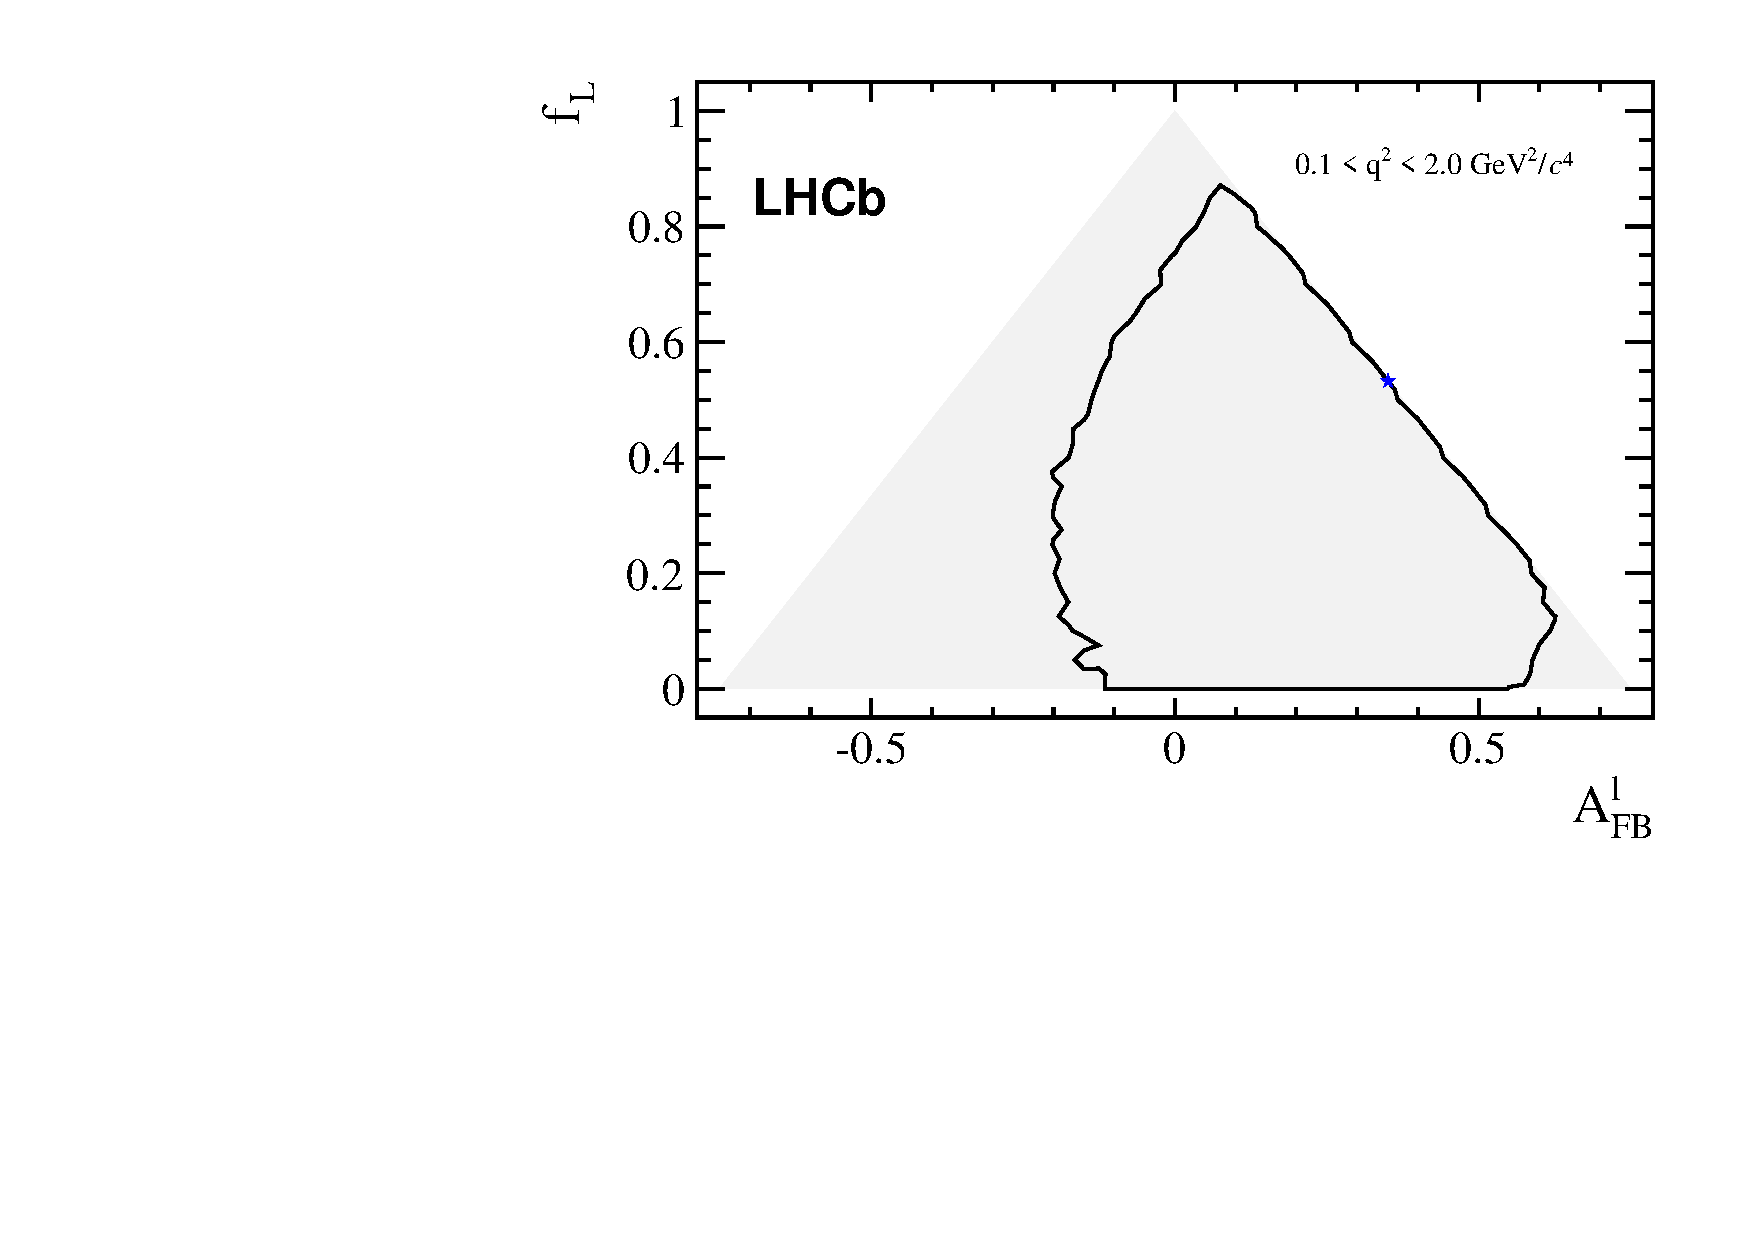
\includegraphics[width=0.45\textwidth]{Lmumu/figs/Contours/contours_010_200_1D.pdf}
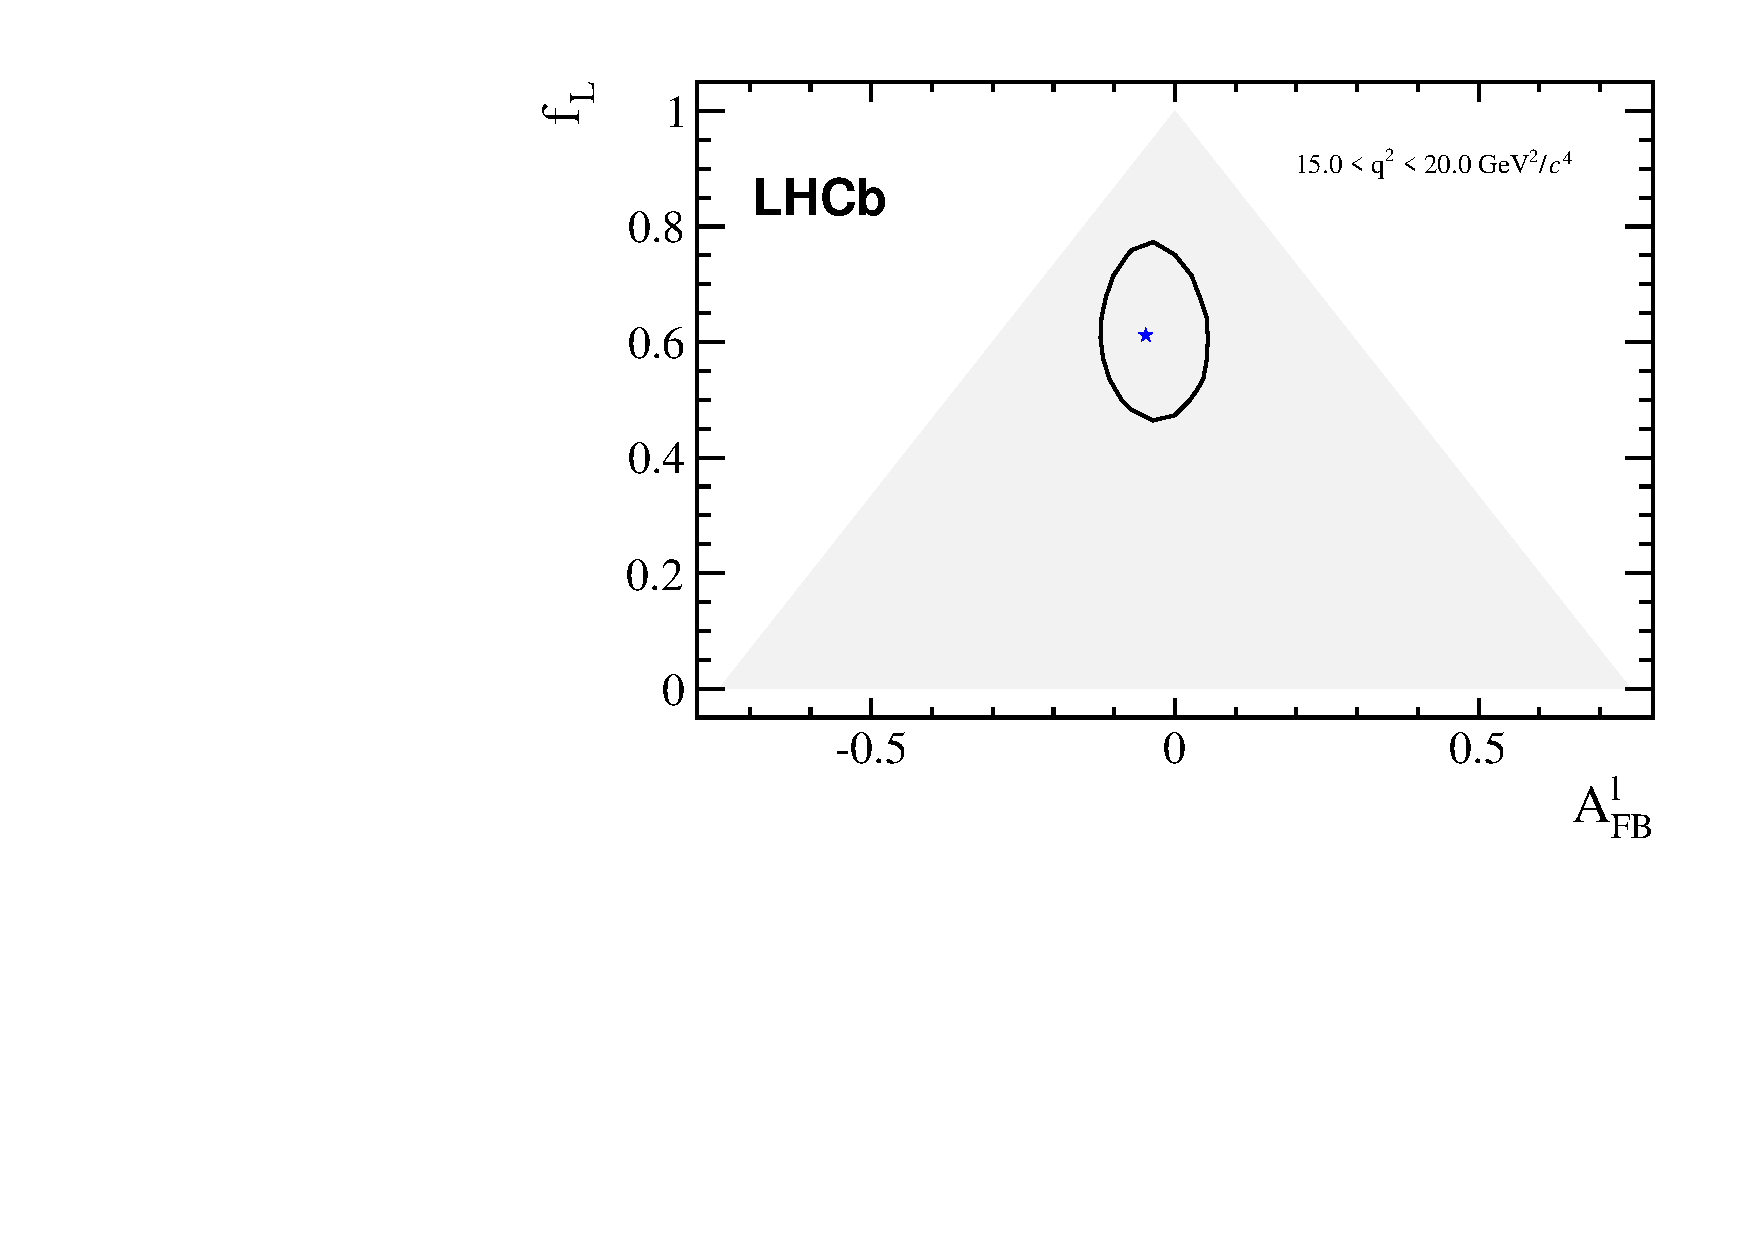
\includegraphics[width=0.45\textwidth]{Lmumu/figs/Contours/contours_1500_2000_1D.pdf}
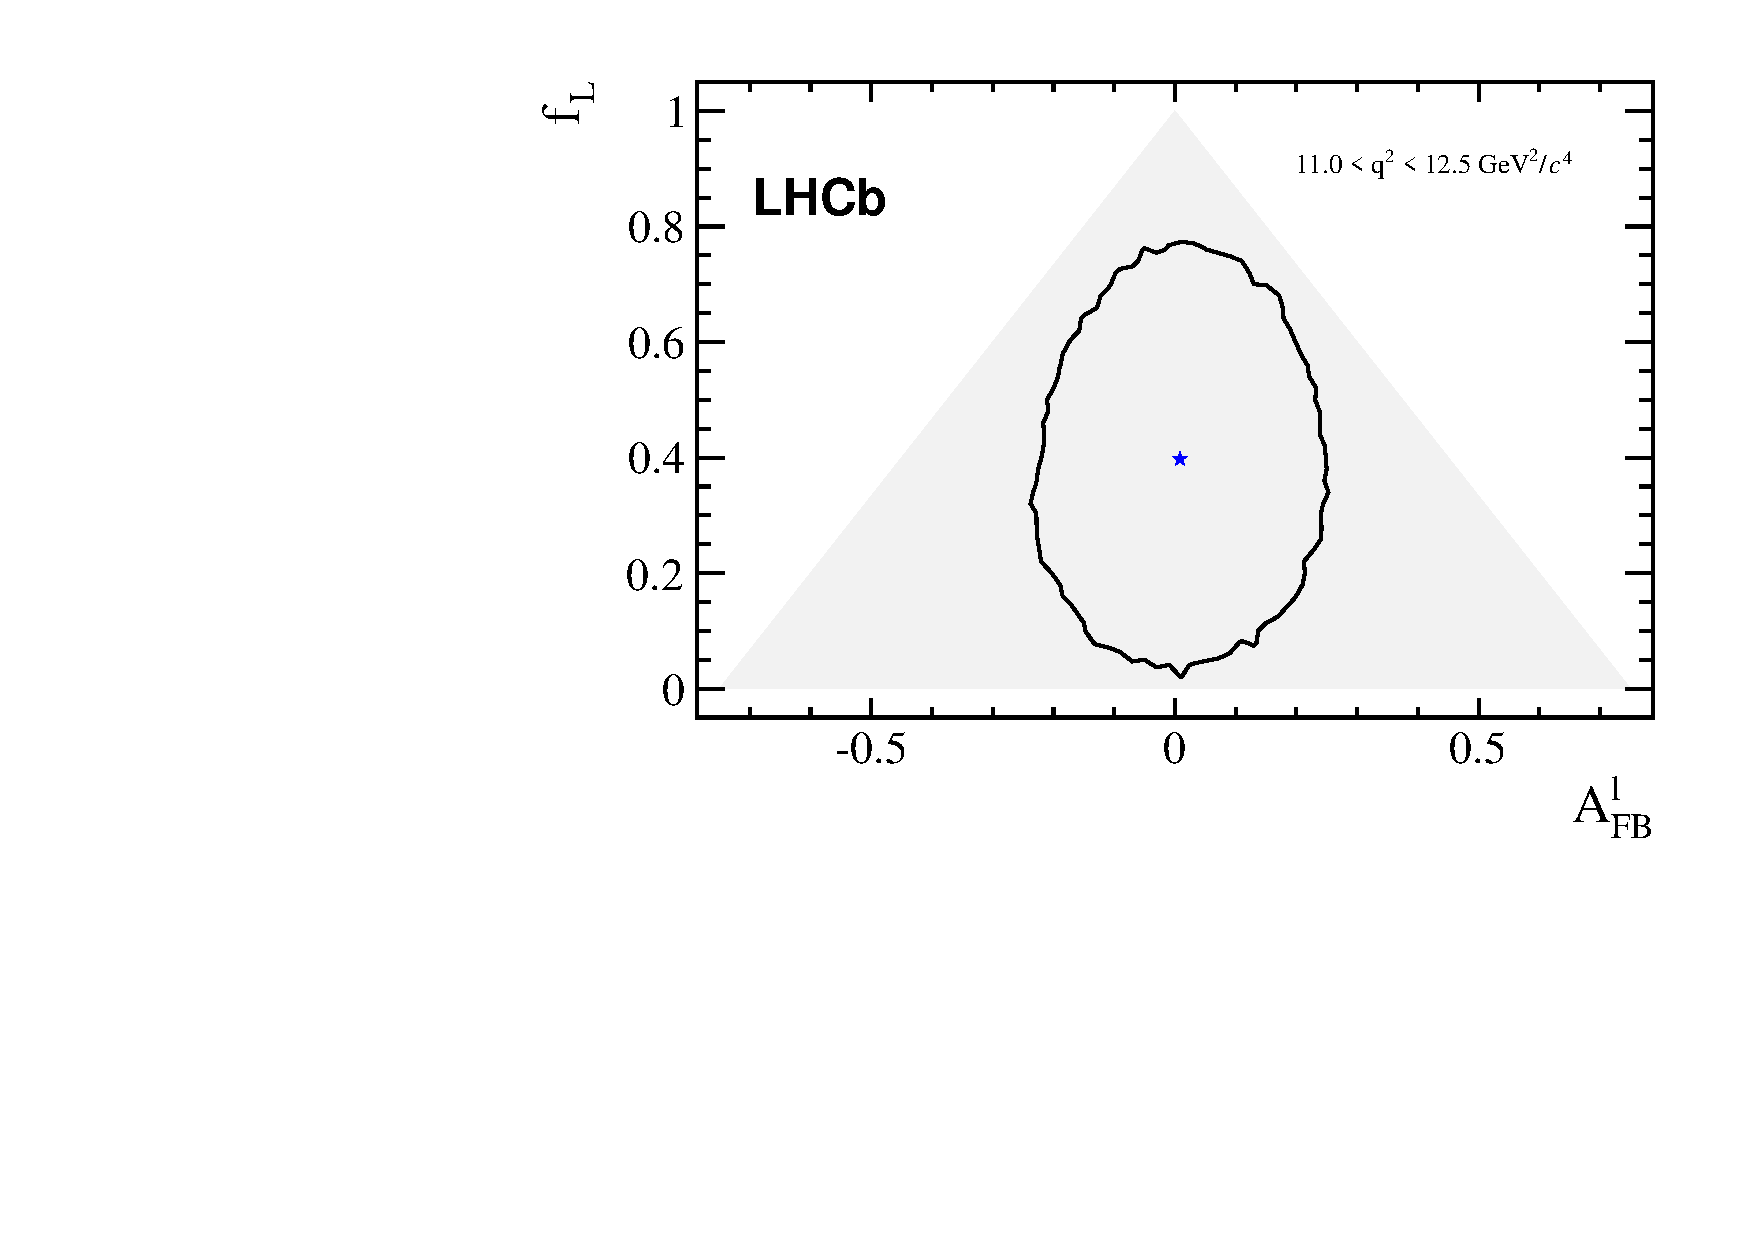
\includegraphics[width=0.45\textwidth]{Lmumu/figs/Contours/contours_1100_1250_1D.pdf}
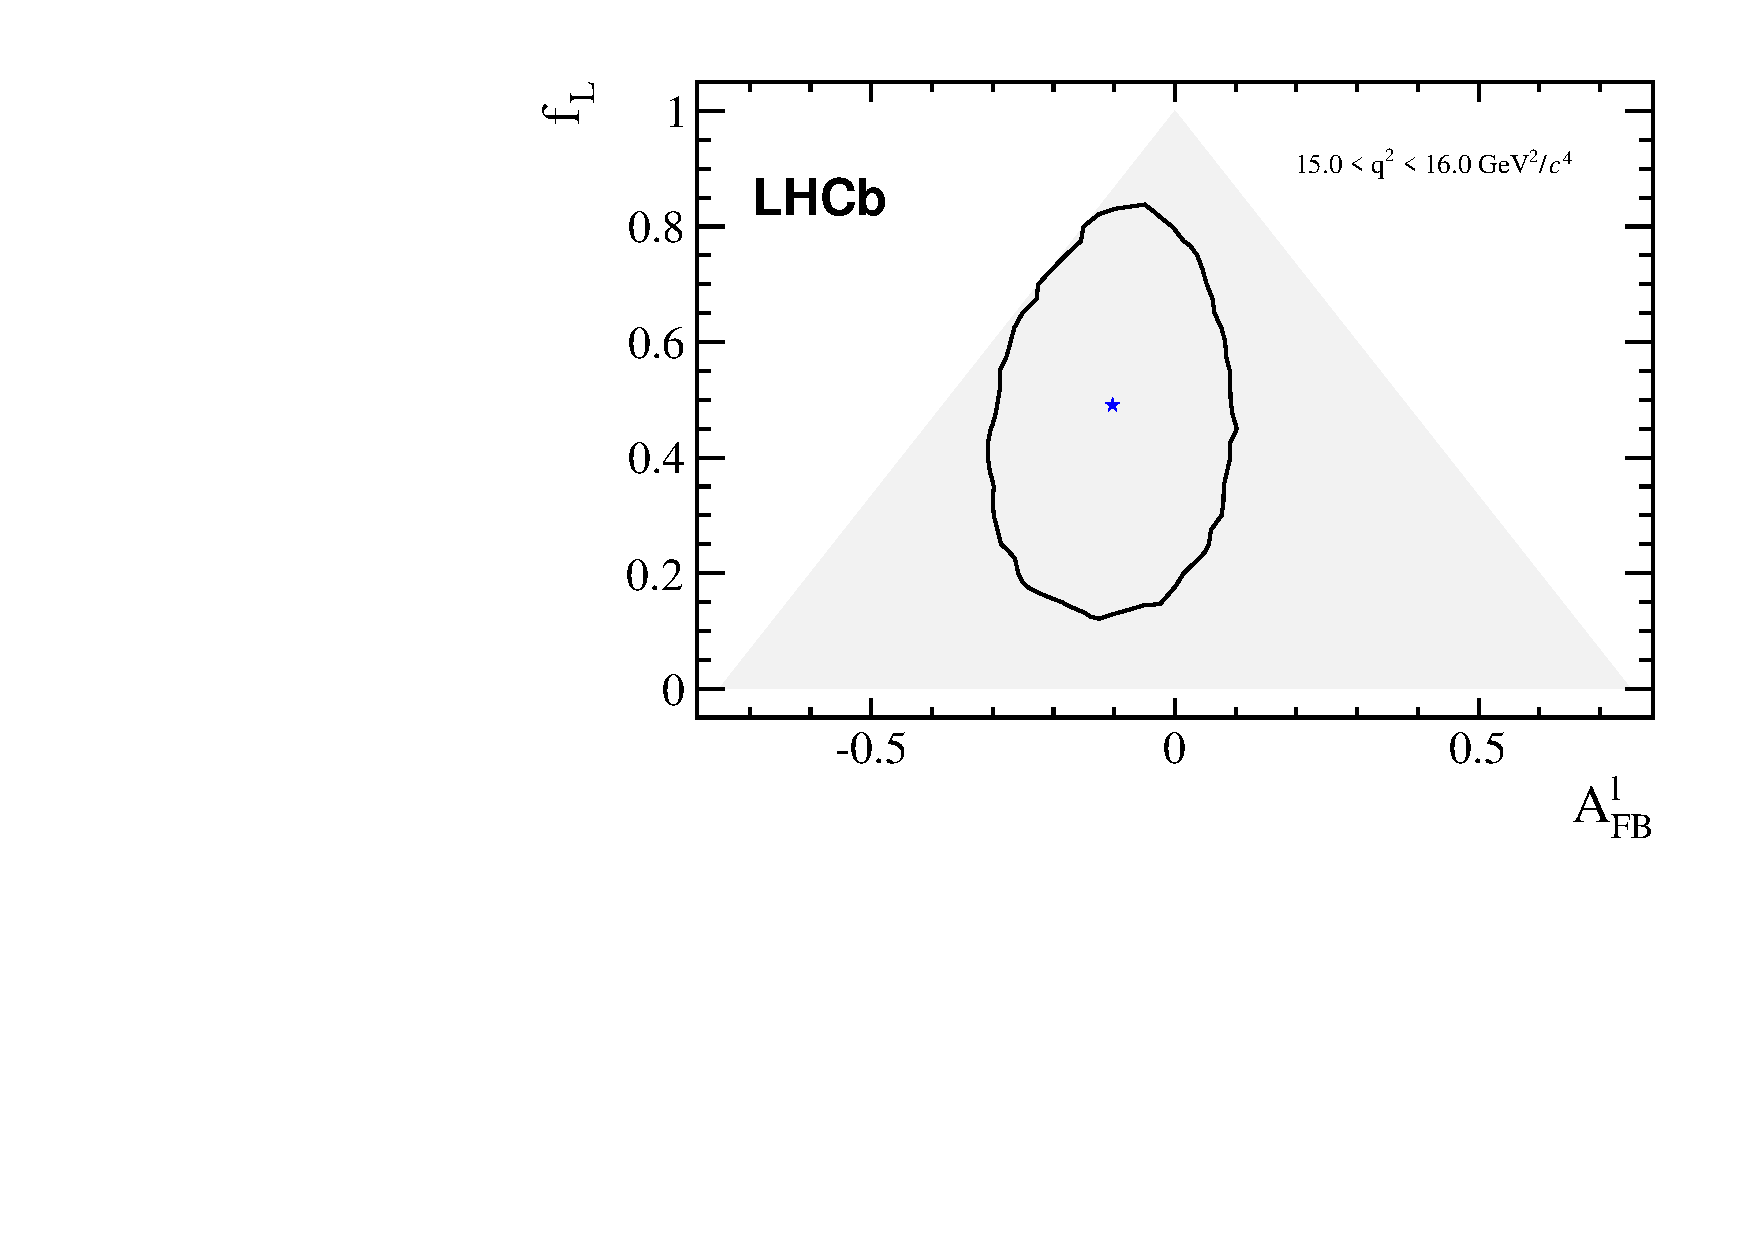
\includegraphics[width=0.45\textwidth]{Lmumu/figs/Contours/contours_1500_1600_1D.pdf}
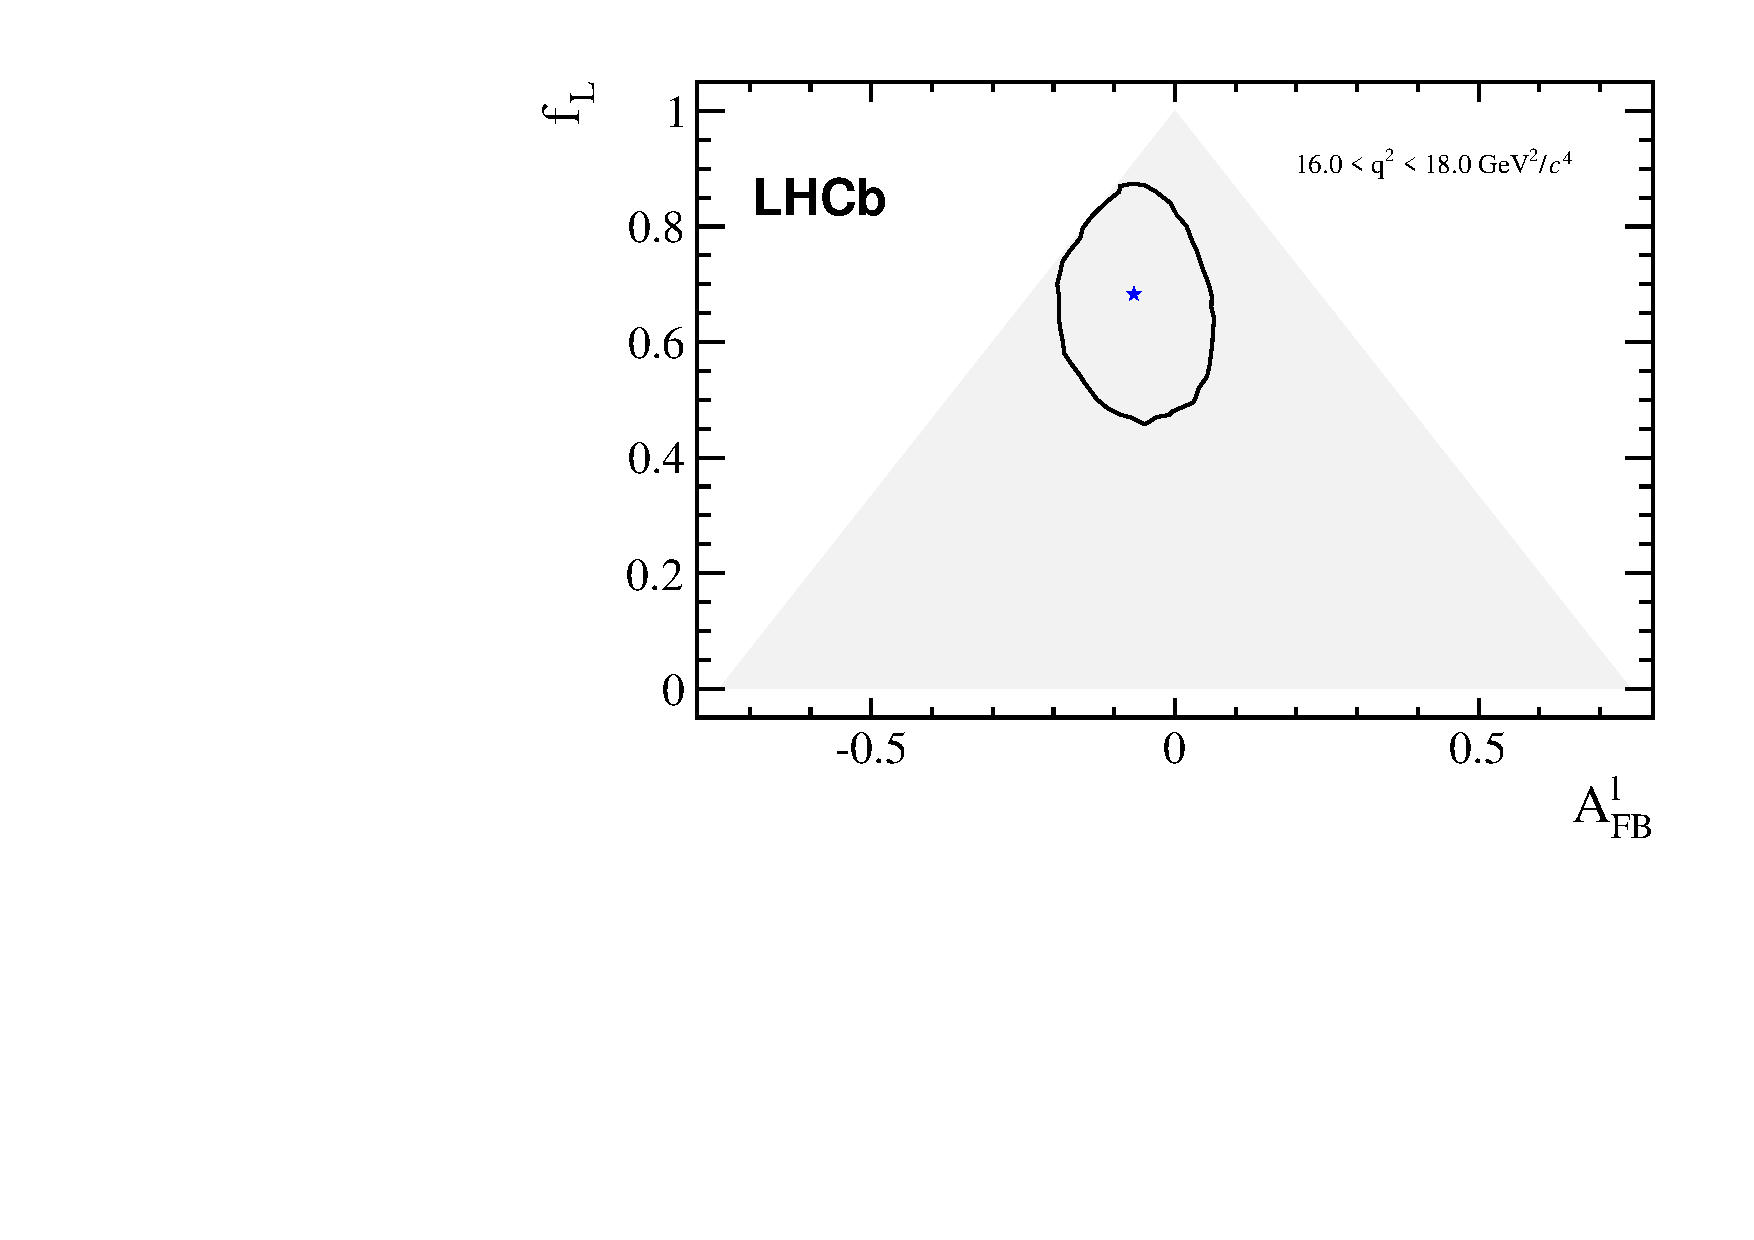
\includegraphics[width=0.45\textwidth]{Lmumu/figs/Contours/contours_1600_1800_1D.pdf}
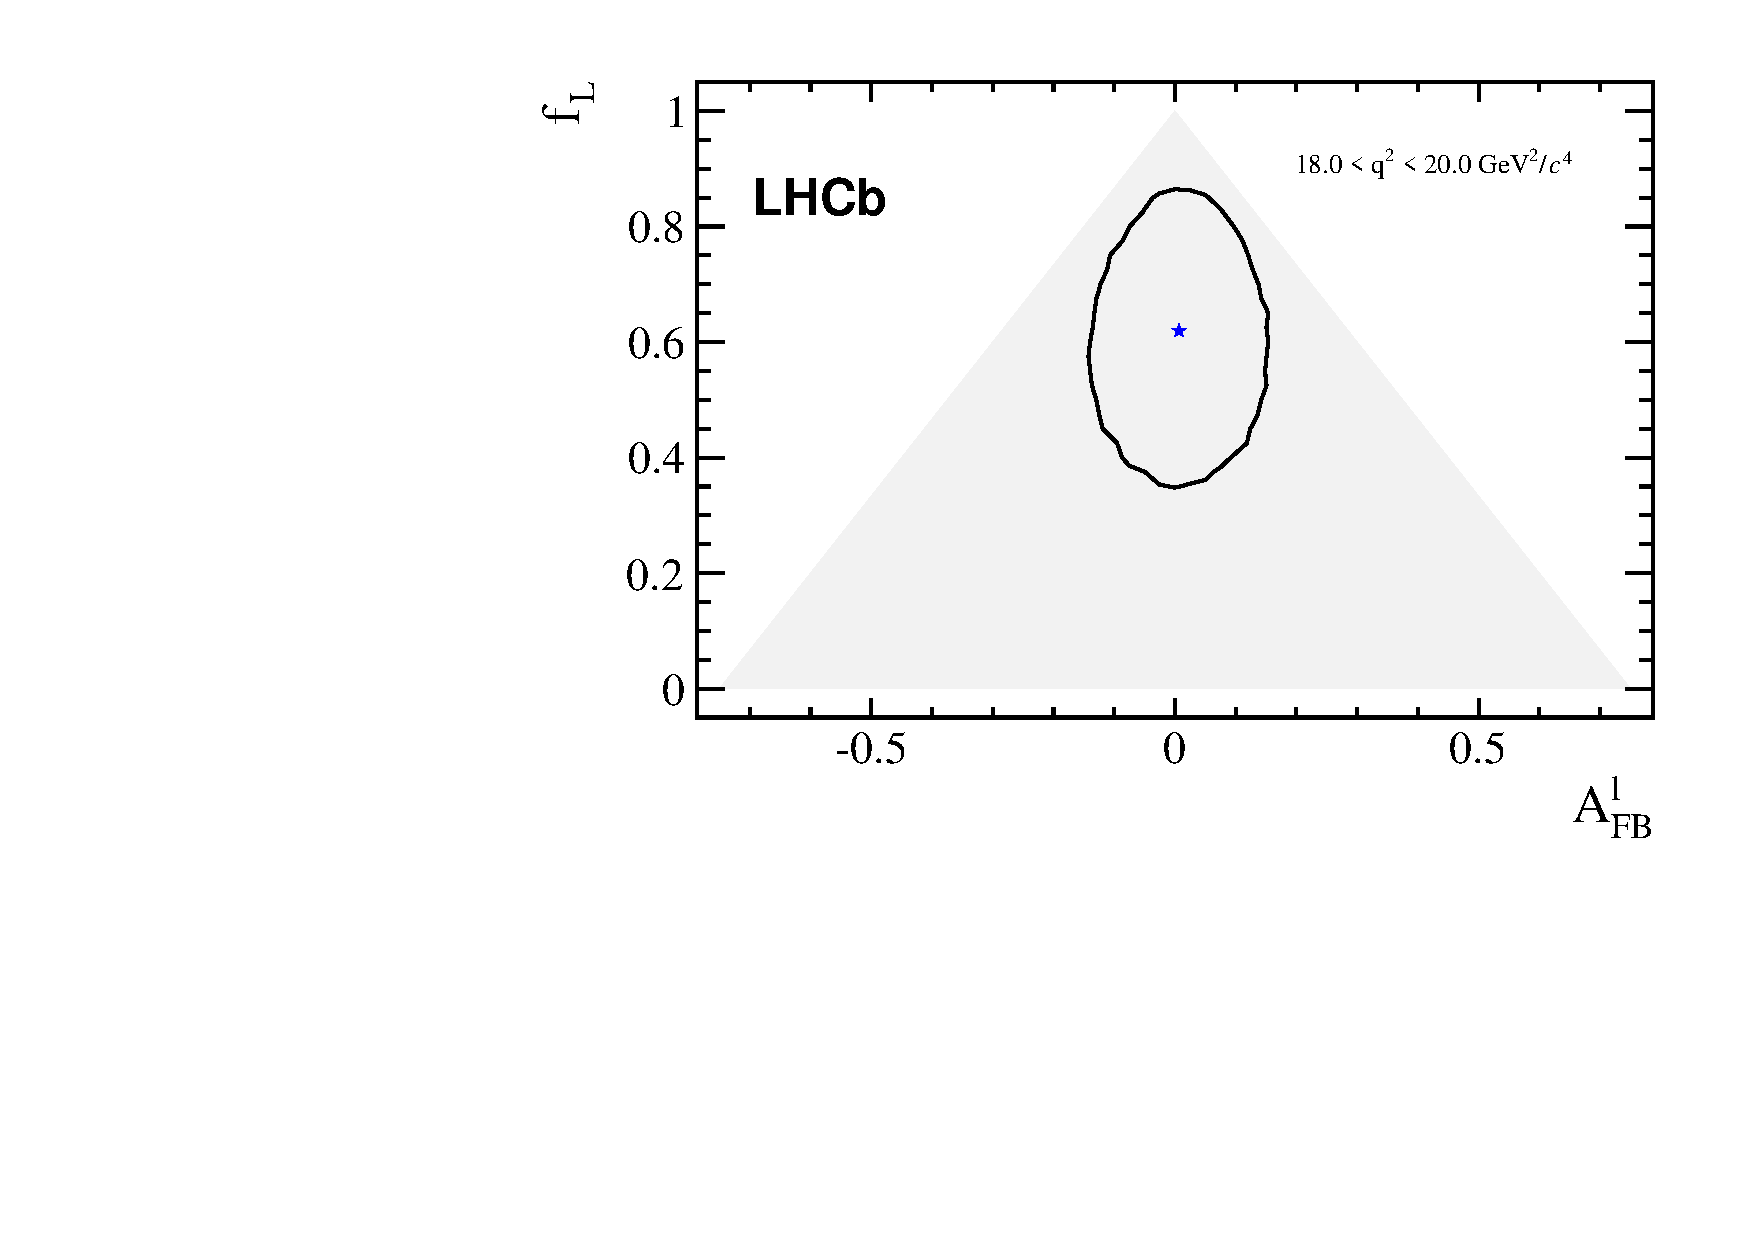
\includegraphics[width=0.45\textwidth]{Lmumu/figs/Contours/contours_1800_2000_1D.pdf}
\caption{In black 2-dimensional 68\% CL confidence regions as a function of $A_{FB}^\ell$ and $f_L$. }
\label{fig:contours}
\end{figure}
